\documentclass[a4paper]{article}

\setlength{\parindent}{0pt}
\setlength{\parskip}{1em}

\pagestyle{headings}

\usepackage{amssymb}
\usepackage{amsmath}
\usepackage{amsthm}
\usepackage{mathtools}
\usepackage{graphicx}
\usepackage{hyperref}
\usepackage{color}
\usepackage{microtype}
\usepackage{tikz}
\usepackage{pgfplots}
\usepackage{pgfplotstable}

\newcommand{\N}{\mathbb{N}}
\newcommand{\Q}{\mathbb{Q}}
\newcommand{\Z}{\mathbb{Z}}
\newcommand{\R}{\mathbb{R}}
\newcommand{\C}{\mathbb{C}}
\newcommand{\D}{\mathcal{D}}
\renewcommand{\S}{\mathcal{S}}
\renewcommand{\P}{\mathbb{P}}
\newcommand{\F}{\mathbb{F}}
\newcommand{\E}{\mathbb{E}}
\newcommand{\bra}{\langle}
\newcommand{\ket}{\rangle}


\graphicspath{{Image/}}

\hypersetup{
    colorlinks=true,
    linktoc=all,
    linkcolor=blue
}

\theoremstyle{definition}
\newtheorem*{axiom}{Axiom}
\newtheorem*{claim}{Claim}
\newtheorem*{conv}{Convention}
\newtheorem*{coro}{Corollary}
\newtheorem*{defi}{Definition}
\newtheorem*{eg}{Example}
\newtheorem*{lemma}{Lemma}
\newtheorem*{notation}{Notation}
\newtheorem*{prob}{Problem}
\newtheorem*{post}{Postulate}
\newtheorem*{prop}{Proposition}
\newtheorem*{rem}{Remark}
\newtheorem*{thm}{Theorem}

\DeclareMathOperator{\vdiv}{div}
\DeclareMathOperator{\grad}{grad}
\DeclareMathOperator{\curl}{curl}
\DeclareMathOperator{\Ann}{Ann}
\DeclareMathOperator{\Fit}{Fit}
\DeclareMathOperator{\Diag}{Diag}
\DeclareMathOperator{\tr}{tr}
\DeclareMathOperator{\im}{im}
\DeclareMathOperator{\Mat}{Mat}
\DeclareMathOperator{\Log}{Log}
\DeclareMathOperator{\Isom}{Isom}
\DeclareMathOperator{\Mesh}{Mesh}
\DeclareMathOperator{\Sym}{Sym}
\DeclareMathOperator{\Aut}{Aut}
\DeclareMathOperator{\cosech}{cosech}
\DeclareMathOperator{\Card}{Card}
\DeclareMathOperator{\Gal}{Gal}


\setcounter{section}{-2}

\begin{document}

\title{Graph Theory}

\maketitle

\newpage

\tableofcontents

\newpage

\section{-1}

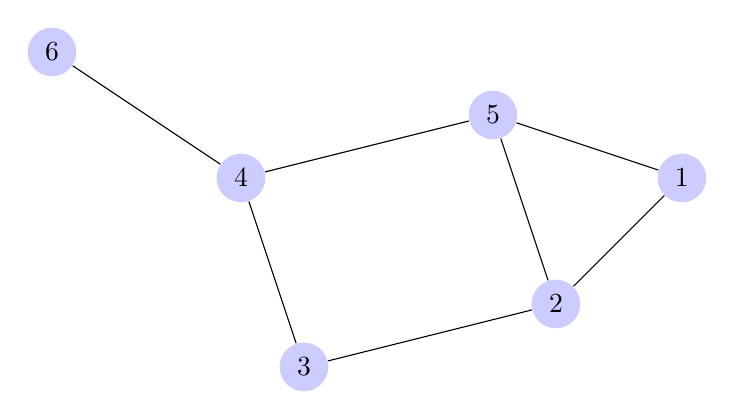
\begin{tikzpicture}
  [scale=.8,auto=left,every node/.style={circle,fill=blue!20}]
  \node (n6) at (1,10) {6};
  \node (n4) at (4,8)  {4};
  \node (n5) at (8,9)  {5};
  \node (n1) at (11,8) {1};
  \node (n2) at (9,6)  {2};
  \node (n3) at (5,5)  {3};

  \foreach \from/\to in {n6/n4,n4/n5,n5/n1,n1/n2,n2/n5,n2/n3,n3/n4}
    \draw (\from) -- (\to);

\end{tikzpicture}

\newpage

\section{Introduction}

Some not very useful examples.

\newpage

\section{Ramsey Theory}

\begin{defi}
A \emph{graph} is an ordered pair $(V,E) = G$ where $V$ is a finite set and $E$ is a set of unordered pairs of distinct elements of $V$. We call elements of $V$ \emph{vertices} of $G$ and elements of $E$ \emph{edges}.

We often write $v \in G$ to mean $v \in V$ and similarly for edges as well. Often we denote $\{u,v\} \in E$ by $uv$.
\end{defi}

\begin{eg}
$G = (\{1,2,3,4,5,6,7\},\{12,23,13,14,67\})$ is a graph. We can represent a graph by a drawing: take a point for each vertex, join two vertices if they are in an edge.

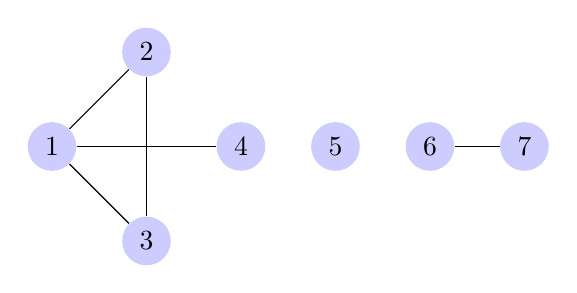
\begin{tikzpicture}
  [scale=.6,auto=left,every node/.style={circle,fill=blue!20}]
  \node (n1) at (0,0) {1};
  \node (n2) at (2,2)  {2};
  \node (n3) at (2,-2)  {3};
  \node (n4) at (4,0) {4};
  \node (n5) at (6,0)  {5};
  \node (n6) at (8,0)  {6};
  \node (n7) at (10,0) {7};

  \foreach \from/\to in {n1/n2,n1/n3,n2/n3,n1/n4,n6/n7}
    \draw (\from) -- (\to);

\end{tikzpicture}

\end{eg}

\begin{defi}
Let $G=(V,E)$ and $G'=(V',E')$ be graphs. An \emph{isomorphism} from $G$ to $G'$ is a bijection $\varphi:V \to V'$ such that for all $u,v\in V$, we have $\phi(u)\phi(v) \in E' \iff uv \in E$.

If such an isomorphism exists, we say $G$ is isomorphic to $G'$.

Suppose also $H = (W,F)$ is a graph. We say $H$ is a \emph{subgraph} of $G$ and write $H \subset G$ if $W \subset V$ and $F \subset E$.

Often we say $H$ is a subgraph of $G$ to mean $H$ is isomorphic to a subgraph of $G$.
\end{defi}

\begin{eg} (Complete graph)\\
The \emph{complete graph of order $n$}, $K_n$, has $n$ vertices with every pair forming an edge.

K1:
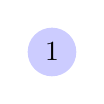
\begin{tikzpicture}
  [scale=.6,auto=left,every node/.style={circle,fill=blue!20}]
  \node (n1) at (0,0) {1};
\end{tikzpicture}
\end{eg}

K3:
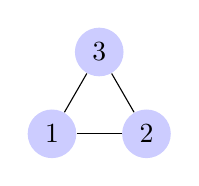
\begin{tikzpicture}
  [scale=.6,auto=left,every node/.style={circle,fill=blue!20}]
  \node (n1) at (0,0) {1};
  \node (n2) at (2,0)  {2};
  \node (n3) at (1,1.732)  {3};

  \foreach \from/\to in {n1/n2,n1/n3,n2/n3}
    \draw (\from) -- (\to);

\end{tikzpicture}

K5:
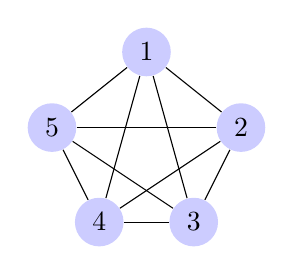
\begin{tikzpicture}
  [scale=.6,auto=left,every node/.style={circle,fill=blue!20}]
  \node (n1) at (0,3.6) {1};
  \node (n2) at (2,2)  {2};
  \node (n3) at (1,0)  {3};
  \node (n4) at (-1,0) {4};
  \node (n5) at (-2,2)  {5};

  \foreach \from/\to in {n1/n2,n1/n3,n2/n3,n1/n4,n2/n4,n3/n4,n1/n5,n2/n5,n3/n5,n4/n5}
    \draw (\from) -- (\to);

\end{tikzpicture}

Note that if $m \leq n$ then $K_m \subset K_n$.

Recall \emph{Schur's Theorem}: Let $k$ be a positive integer. Then there is a positive integer $n$ s.t. if the set $[n] = \{1,2,...,n\}$ is coloured with $k$ colours, we can find $a,b,c$ with $a+b = c$ and $a,b,c$ the same colour. An idea to prove this in graph theory is to consider vertices as numbers, edges as difference between two vertices, and we try to colour the edges.

For example, suppose the edges of complete graph $K_6$ are coloured blue/yellow. Then we can find a monochromatic triangle. Note that Schur's Theorem for $k=2$ follows immediately. In this graph form of the problem statement, statement for more colours is amenable to an induction proof.

\begin{prop}
Let $k$ be a positive integer. Then there is a positive integer $n$ s.t. whenever the edges of $K_n$ are coloured with $k$ colours, we can find a monochromatic triangle.
\begin{proof}
We use induction on $k$. $k=1$ is trivial with $n=3$.
For $k>1$, by induction hypothesis we can find a $m$ s.t. for any $K_m$ coloured with $(k-1)$ colours, there exist a monochromatic triangle.\\
Let $n=k(m-1)+2$. Now $k$-colour the edges of $K_n$. Pick vertex $v$. The number of edges containing $v$ is $n-1=k(m-1)+1$, so some $m$ of them are the same colour, wlog blue. Now let $H$ be a $K_m$ joined to $v$ by blue edges. If $H$ contains a blue edge then we have a blue triangle. Otherwise $H$ is only coloured with at most $k-1$ colours, and from the induction hypothesis we know that there is a monochromatic triangle in that $K_m$.
\end{proof}
\end{prop}

\begin{rem}
We can also try to get an explicit upper bound from what we proved above. Let $f(k)$ be the smallest $n$ that works with $k$ colours. Clearly $f(1) = 3$. The proof says for $k>1$, $f(k) \leq k(f(k-1)-1)+2 \leq kf(k-1)$. So by induction we have $f(k) \leq 3k!$ for all $k$.
\end{rem}

\begin{rem}
Schur's Theorem follows immediately if we consider the graph approach of the problem.
\end{rem}

Another problem that arises naturally is that, can we find larger monochromatic subgraphs, e.g. a $K_4$? We can think about the two colours case first for simplicity -- the answer is yes, but it requires some intermediate step.

\begin{eg}
Let $K_{10}$ have edges coloured blue/yellow. Then there is a blue triangle or yellow $K_4$.
\begin{proof}
Take a vertex $v$. It's degree 9, so either $v$ has 4 blue edges, in which case there is a blue triangle or yellow $K_4$; otherwise $v$ has 6 yellow edges, in which case there is a blue or yellow triangle within it, together with $v$ we have either a blue triangle or yellow $K_4$.
\end{proof}
\end{eg}

\begin{prop}
Let $K_{20}$ be coloured blue/yellow. Then there exists a monochromatic $K_4$.
\begin{proof}
Pick a vertex $v$. It's degree 19 so 10 of them are the same colour, wlog blue. Then by the previous example we get the desired result immediately.
\end{proof}
\end{prop}

Now we are interested in a more general problem.

\begin{defi}
Let $s,t \geq 2$. The \emph{Ramsey number} $R(s,t)$ is the least $n$ s.t. whenever $K_n$ has edges coloured blue or yellow, ther must be a blue $K_s$ or a yellow $K_t$, provided if such an $n$ exists. Also we write $R(s) = R(s,s)$ for simplicity.
\end{defi}

Earlier we've seen $R(3) = 6$, $R(3,4) \leq 10$, $R(4) \leq 20$.

\begin{thm} (Ramsey's theorem)\\
$R(s,t)$ exists for all $s,t \geq 2$. Moreover, is $s,t > 2$, then $R(s,t) \leq R(s-1,t)+R(s,t-1)$.
\begin{proof}
We'll prove by induction on $s+t$.

First consider the case $s=2$: Obviously $R(2,t)=t$. The case $t=2$ is symmetric.

Now if $s,t>2$, Let $a=R(s-1,t)$ and $b=R(s,t-1)$ (and we know by induction hypothesis that these exist).

Now let $n=a+b$, and we colour edges of $K_n$ by blue and yellow. Pick $v\in K_n$, it has either $a$ blue or $b$ yellow edges. Then we can just apply the induction hypothesis.
\end{proof}
\end{thm}

And we have an immediate corollary:

\begin{coro}
For all $s,t \geq 2$, $R(s,t) \leq 2^{s+t}$. So $R(s) \leq 4^s$.
\begin{proof}
We induct on $s+t$. The case $s=2$ or $t=2$ is obvious. For $s,t>2$ we have
\begin{equation*}
\begin{aligned}
R(s,t) &\leq R(s-1,t) + R(s,t-1)\\
&\leq 2^{s-1+t}+2^{s+t-1}\\
&=2^{s+t}.
\end{aligned}
\end{equation*}
\end{proof}
\end{coro}

We can prove that $R(s) = O\left(\frac{4^s}{\sqrt{s}}\right)$ by the same proof but more carefully -- this was first proved in 1935. After 50 years we proved that $R(s) = O\left(\frac{4^s}{s}\right)$ by being very clever and working hard. After another 20 years (2009), by being even more careful and working harder, we can prove $R(s) = O\left(\frac{4^s}{s^k}\right)$ for any $k$. It is still unknown that if the base in the expression can be reduced by any tiny amount.

\begin{thm} (Multi-colour Ramsey Theorem)\\
Let $k \geq 1$ and $s \geq 2$. Then there exists some $n$ s.t. whenever the edges of $K_n$ coloured with $k$ colours, we can find a monochromatic $K_s$.
\begin{proof}
Use induction on $k$. For $k=1$ we just take $n=s$.

Now let $k>1$. By induction hypothesis, we can find $M$ s.t. $K_m$ coloured with $(k-1)$ colours contain a monochromatic $K_s$. Now let $n=R(s,m)$ and colour $K_n$ with $k$ colours, including blue but not yellow. Now we re-colour by turning all the non-blue edges yellow. Now by definition of $n$ we have either a blue $K_s$, in which case we're done, or we have a yellow $K_m$. But that means we have a $K_m$ coloured with $k-1$ colours, which by induction hypothesis we can also find a monochromatic $K_s$.
\end{proof}
\end{thm}

\begin{rem}
We write $R_k(s)$ for the smallest $n$ that works. In particular, $R_1(s) = s$, $R_2(s) = R(s)$. Proof of the above theorem will give $R_k(s) \leq 4^{s^{k-1}}$ (see example sheet 1).
\end{rem}

\begin{rem}
What we really mean by colouring is that we have a function $c:E \to [k] = \{1,2,...,k\}$. 'Blue' and 'yellow' are just arbitrary names of the colours.

We say $H=(W,F)$ is monochromatic if $c|_F$ is a constant.
\end{rem}

With any number of colours, we can find arbitrarily large monochromatic subgraphs. What about infinite ones?

\begin{defi}
An infinite graph is an ordered pair $G=(V,E)$ where $V$ is an infinite set and $E$ is a set of unordered pairs of distinct elements of $V$. Note that in our terminology, an infinite graph is \emph{not} a graph.
\end{defi}

We should also let a possibly infinite graph mean a graph or an infinite graph.

The \emph{infinite complete graph}, $K_\infty$, will mean the infinite graph with a \emph{countably} infinite vertex set and every pair of vertices forming an edge.

Where it makes sense to do so, we carry terminology over from graphs to infinite graphs.

Suppose edges of $K_\infty$ are coloured blue or yellow. What can we find? By Ramsey, we can find a monochromatic $K_s$ for every finite $s=1,2,3,...$. This doesn't imply we find an infinite monochromatic subgraph.

\begin{thm} (5, Infinite Ramsey Theorem)\\
Let $k \geq 1$. Whenever the edges of $K_\infty$ are $k$-coloured, we have a monochromatic $K_\infty$ as a subgraph.
\begin{proof}
Take $v_1 \in K_\infty$. The vertex $v_1$ is infinitely many edges, so infinitely of them are the same colour. Let $A_1 \subset V$ be the infinite subset of vertices of $K_\infty$ s.t. for all $u \in A_1$, $v_1 u$ has colour $c_1$.

Now pick $v_2 \in A_1$. Similarly, we can find an infinite $A_2 \subset A_1$ s.t. all edges $v_2,u(u \in A_2$) have colour (WLOG) $c_2$. Keep going and we get infinite sequences $v_1,v_2,v_3,...$ of vertices, $c_1,c_2,c_3,...$ of colours and $A_1 \supset A_2 \supset A_3 \supset ...$ of infinite sets s.t.\\
$\bullet$ for $i \geq 2$, $v_i \in A_{i-1}$;\\
$\bullet$ for $i \geq 1$, for all $u \in A_i$, $v_i u$ is an edge of colour $c_i$.

In particular, if $i<j$ then $v_i v_j$ has colour $c_i$. However there are only finitely many colours. So infinitely many of the $c_i$ are the same, say we have $c_{i_1} = c_{i_2} = ... $. Then $v_{i_1},v_{i_2},...$ form a monochromatic $K_\infty$.
\end{proof}
\end{thm}

An application of the above theorem is

\begin{coro} (6, Bolzano-Weierstrass Theorem)\\
Any bounded sequence has a convergent subsequence (apparently, in a sequentially compact space).
\begin{proof}
Any bounded monotonic sequence converges, so it's enough to show that any real sequence $(x_n)_{n \geq 1}$ has a monotonic subsequence. Let $G$ be a $K_\infty$ with vertex set $\{1,2,3,...\}$. Colour $ij$ ($i<j$) blue if $x_i<x_j$, and yellow otherwise. By theorem 5 there is a monochromatic subgraph isomorphic to $K_\infty$, so there is a monotonic subsequence.
\end{proof}
\end{coro}

\newpage

\section{Basic Terminology}
Let $G=(V,E)$ be a graph. Sometimes we write $V(G) = V$ and $E(G) = E$.

The \emph{order} of $G$ is $|G| = |V(G)|$. We denote the number of edges of $G$ by $e(G)=|E(G)|$, sometimes this is called the 'size' of $G$.

Now let $v \in G$. The \emph{neighbourhood} of $v$ is the set $\Gamma(v) = \{w \in G: vw \in E(G)\}$.

If $w \in \Gamma(v)$ then $w$ is a \emph{neighbour} of $v$, or $w$ is \emph{adjacent} to $v$, written as $w \sim v$.

The \emph{degree} of $v$ is $d(v) = |\Gamma(v)|$, i.e. the number of vertices adjacent to $v$. From this it should be obvious what the maximum degree, minimum degree, and average degree mean. We denote the maximum and minimum degree by $\Delta(G)$, $\delta(G)$ respectively.

Clearly $\delta(G) \leq $average degree $\leq \Delta(G)$. If every vertex in $G$ has the same degree, we say $G$ is \emph{regular}. If this degree is $r$, we say $G$ is $r-$regular.

\begin{eg}
Each edge contributes 2 to the sum of degrees, so we know $2e(G)$ is equal to $\sum_{v \in G} d(v)$.
\end{eg}

Let $G$ be a graph. A \emph{path} in $G$ is a finite sequence $v_0,...,v_l$ of distinct vertices of $G$ with $v_{i-1} \sim v$ for $1 \leq i \leq l$. We say this path has length $l$ and goes from $v_0$ to $v_l$. We write $v \to w$ to mean there is a path from $v$ to $w$. The relation $\to$ is an equivalence relation. The equivalence classes of $\to$ are called the \emph{components} of $G$. If $G$ has only one component, we say $G$ is \emph{connected}.

A \emph{cycle} is a sequence $v_0,...,v_l$ of vertices of $G$ with $v_0,...,v_{l-1}$ distinct, $v_l = v_0$, $v_{i-1} \sim v_i$ for $1 \leq i \leq l$, and $l \geq 3$. We say the length of the cycle is $l$. 

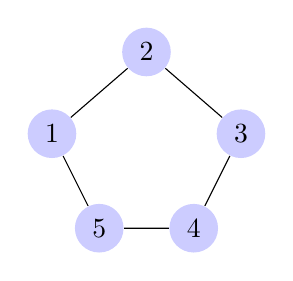
\begin{tikzpicture}
  [scale=.6,auto=left,every node/.style={circle,fill=blue!20}]
  \node (n1) at (0,0) {1};
  \node (n2) at (2,1.73)  {2};
  \node (n3) at (4,0)  {3};
  \node (n4) at (3,-2) {4};
  \node (n5) at (1,-2)  {5};

  \foreach \from/\to in {n1/n2,n2/n3,n4/n3,n5/n4,n1/n5}
    \draw (\from) -- (\to);

\end{tikzpicture}

A graph with no cycles is called a \emph{forest}. A \emph{tree} is a connected forest. Each component of a forest is a tree.

Suppose $G,H$ are graphs with $V(G) \cap V(H) = \phi$. The \emph{disjoint union} of $G,H$ is the graph $G \cup H$, with $V(G\cup H) = V(G) \cup V(H)$ and $E(G\cup H) = E(G) \cup E(H)$.

Often we write $G \cup H$ even if $V(G) \cap V(H) \neq \phi$. This means that we take graphs $G',H'$ that are isomorphic to $G$ and $H$, s.t. $V(G') \cap V(H') = \phi$, then take $G' \cup H'$.

\begin{eg}
(i) $K_3 \cup K_5$:

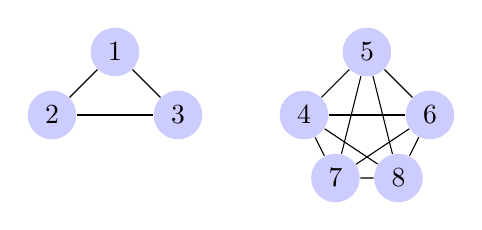
\begin{tikzpicture}
  [scale=.8,auto=left,every node/.style={circle,fill=blue!20}]
  \node (n1) at (1,1) {1};
  \node (n2) at (0,0)  {2};
  \node (n3) at (2,0)  {3};
  \node (n4) at (4,0) {4};
  \node (n5) at (5,1)  {5};
  \node (n6) at (6,0)  {6};
  \node (n7) at (4.5,-1)  {7};
  \node (n8) at (5.5,-1)  {8};

  \foreach \from/\to in {n1/n2,n1/n3,n2/n3,n4/n5,n4/n6,n4/n7,n4/n8,n5/n6,n5/n7,n5/n8,n6/n7,n6/n8,n7/n8}
    \draw (\from) -- (\to);

\end{tikzpicture}

(ii) Any graph is the disjoint union of its components. For example, a forest is a disjoint union of trees.
\end{eg}

Let $G = (V,E)$ be a graph and let $W \subset V$. The \emph{induced subgraph on $W$} is the graph $G[W]$ with $V(G[W]) = W$ and, for $x,y \in W$, $xy \in E(G[W]) \iff xy \in G$.

Let $G = (V,E)$ be a graph. The \emph{complement} of $G$ is the graph $\bar{G}$ with $V(\bar{G}) = V$ and for distinct $x,y \in V$, $xy \in E(\bar{G}) \iff xy \not\in E$.

\begin{eg}
$\bullet$ Suppose edges of $Kn$ are coloured blue/yellow. We can just think about the 'blue subgraph' with $n$ vertices and blue edges only. The complement is then the yellow subgraph.\\
$\bullet$ For example, consider graph $G$

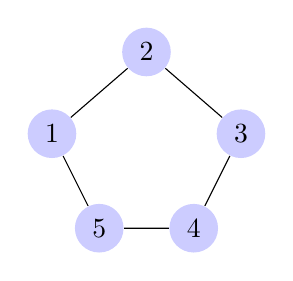
\begin{tikzpicture}
  [scale=.6,auto=left,every node/.style={circle,fill=blue!20}]
  \node (n1) at (0,0) {1};
  \node (n2) at (2,1.73)  {2};
  \node (n3) at (4,0)  {3};
  \node (n4) at (3,-2) {4};
  \node (n5) at (1,-2)  {5};

  \foreach \from/\to in {n1/n2,n2/n3,n4/n3,n5/n4,n1/n5}
    \draw (\from) -- (\to);

\end{tikzpicture}

Then we have $\bar{G}$ is

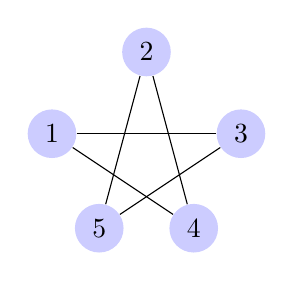
\begin{tikzpicture}
  [scale=.6,auto=left,every node/.style={circle,fill=blue!20}]
  \node (n1) at (0,0) {1};
  \node (n2) at (2,1.73)  {2};
  \node (n3) at (4,0)  {3};
  \node (n4) at (3,-2) {4};
  \node (n5) at (1,-2)  {5};

  \foreach \from/\to in {n1/n3,n2/n4,n3/n5,n4/n1,n2/n5}
    \draw (\from) -- (\to);

\end{tikzpicture}

and by relabelling the vertices we can see that $G$ is actually isomorphic to its complement.

\end{eg}

Reminder of $O$ notation: Let $f,g: \N \to (0,\infty)$. We say $f = O(g)$ if $f<Ag$ for some constant, say $f=\Omega(g)$ if $g=O(f)$, say $f=\Theta(g)$ if $f=O(g)$ and $f=\Omega(g)$. Also, $f=o(g)$ means $f/g \to 0$ (as $n \to \infty$), $f=\omega(g)$ means $f/g \to \infty$, and $f \sim g$ means $f/g \to 1$.

\newpage

\section{Extremal Graph Theory}
Problem 1 (from chapter 1): How large must $n$ be so that if edges of $K_n$ coloured blue/yellow then we always get a monochromatic $K_s$? We can actually let $G$ be the blue subgraph of $K_n$, then $K_n$ has a blue $K_s$ is equivalent to $K_s \subset G$, and $K_n$ has a yellow $K_s$ is equivalent to $G$ has an induced $\bar{K}_s$ subgraph. Then we can rephrase the problem as: How large must $n$ be to force every subgraph of order $n$ to have $K_s$ or $\bar{K}_s$ as an induced subgraph?

Typical example of an extremal problem: how large must some parameter of $G$ be to force $G$ to have a certain property? Alternatively, how big can the parameter be with $G$ not having the property?

\subsection{The Forbidden Subgraph Problem}
Fix a graph $H$ with at least one edge. Let $n \geq |H|$. Clearly $H \subset K_n$ but $H \not\subset \bar{K}_n$. How many edges must a graph $G$ of order $n$ have to force $H \subset G$? Alternatively, if $|G| = n$ and $H \subseteq G$, how large can $e(g)$ be?

\begin{defi}
Define
\begin{equation*}
\begin{aligned}
ex(n,H) = \max\{e(G):|G|=n,H \not\subset G\}
\end{aligned}
\end{equation*}
Problem: can we determine $ex(n,H)$?
\end{defi}

\subsubsection{Triangles}
We want $G$ with $|G|=n$, $e(G)$ large, and $\triangle \not\subset G$. The idea is to have a \emph{bipartite graph}, where we can partition the graph $G$ into two parts $X$ and $Y$ such that there is no edge within $X$ or $Y$ themselves, i.e. with all the edges going from $X$ to $Y$. We define this more properly:

\begin{defi} (Bipartite graph)\\
A graph $G$ is \emph{bipartite} (with bipartition $(X,Y)$) if $V(G)$ can be partitioned as $X \cup Y$ in such a way that if $e \in E(G)$, then $e = xy$ for some $x \in X, y \in Y$.
\end{defi}

Bipartite graphs have no triangles (and indeed no cycles of odd length). In fact, the converse is true.

\begin{thm} (7)\\
A graph is bipartite iff it contains no odd cycles. The proof is an exercise for now.
\end{thm}

However, which bipartite graph is the best? Clearly we want to include all possible edges from $X$ to $Y$.

\begin{defi}
Let $s,t \geq 1$. The complete bipartite graph $K_{s,t}$ has bipartition $(X,Y)$ with $|X| = s$, $|Y| = t$ and $xy \in E(K_{s,t})$ $\forall x \in X, y \in Y$.
\end{defi}

We have $|K_{s,t}| = s+t$ and $e(K_{s,t}) = st$. So we just have to maximize $s(n-s)$. Now we'll prove that no other graphs can beat bipartite graphs.

\begin{thm} (Mantel's theorem)\\
Let $n \geq 3$. Suppose $|G| = n$, $e(G) \geq [\frac{n^2}{4}]$ and $G$ does not contain a triangle. Then $G \cong K_{\lceil \frac{n}{2} \rceil, \lfloor \frac{n}{2} \rfloor}$.
\begin{proof}
By induction. For $n=3$ it's trivial.\\
For $n>3$, let $|G| = n$, $e(G) \geq \lceil \frac{n^2}{4} \rceil$, and $G$ does not contain a triangle. First, remove edges from $G$ if necessary to get $H$ with $|H| = n$, $e(H) = \lfloor \frac{n^2}{4} \rfloor$. Clearly $H$ does not contain a triangle. Let $v \in H$ with $d(v) = \delta(H)$ and let $K = H-v$, i.e. $H$ with vertex $v$ and all edges including $v$ removed. (recall that $\delta(H)$ is the minimum degree). Now $|K|$ = n-1, $K$ does not contain a triangle, and $e(K) = \lfloor \frac{n^2}{4} \rfloor - \delta(H)$.

Suppose $n$ is even. Then $\delta(H)<$average degree of $H = 2e(H)/|H| = n^2/2/n = n2$, hence
\begin{equation*}
\begin{aligned}
e(K) \geq \frac{n^2}{4} - \frac{n}{2} = \frac{(n-1)^2}{4} = \lfloor \frac{(n-1)^2}{4}\rfloor
\end{aligned}
\end{equation*}
Similarly if $n$ is odd we also get $e(K) \geq \lfloor \frac{(n-1)^2}{4} \rfloor$. Hence by induction hypothesis, $K \cong K_{\lceil \frac{n-1}{2} \rceil, \lfloor \frac{n-1}{2} \rfloor}$.

Also, $d(v) = e(H) -e(K)$. If $n$ is even then $d(v) = n/2$. $H$ is formed by adding a vertex $v$ to $K \cong K_{\frac{n}{2},\frac{n-2}{2}}$, and joining $v$ to $n/2$ vertices of $K$ without creating a triangle. If $K$ has bipartition $(X,Y)$, $v$ cannot be joined both to a vertex in $X$ and a vertex in $Y$. So $v$ must be joined to all vertices in the larger of $X,Y$. Thus $H \cong K_{\lceil n/2 \rceil, \lfloor n/2 \rfloor}$, and similar if $n$ is odd. We recover $G$ by adding edges to $H$ without making a triangle. But any new edge creates a triangle, so $G \cong H$.
\end{proof}
\end{thm}

Hence if $|G| = n, e(G) > \lfloor \frac{n^2}{4}\rfloor$, then $G$ contains a triangle. Therefore $ex(n,\triangle) = \lfloor\frac{n^2}{4}\rfloor$.

\subsubsection{Complete graphs}

Last time we considered $K_3$, the triangle. What about $K_4$? We can try something like a 'tripartite graph'. Formally,

\begin{defi}
A graph $G$ is $\$r$-partite if we can partition $V(G) = X_1 \cup ... \cup X_r$ in such a way that if $xy \in E(G)$, then $x \in X_i, y \in X_j$ for some $i,j$ with $i \neq j$.\\
We say $G$ is complete $r$-partite graph if whenever $x \in X_i$, $y \in X_j$ with $i \neq j$, we have $xy \in E(G)$.\\
The Turan graph $T_r(n)$ is the complete $r$-paritte graph with $n$ vertices and vertex-classes as equal as possible. We write $t_r(n) = e(T_r(n))$.
\end{defi}

Properties of the Turan graph:

$\bullet$ $K_{r+1} \not\subset T_r(n)$. If we add an edge to $T_r(n)$, we create a $K_{r+1}$.

\subsubsection{Bipartite graphs}

\begin{eg}
What is $ex(n,C_4)$? Note that $C_4 \cong K_{2,2}$. \\
$C_4$ is made from two copies of $P_2$. Suppose $G$ is a graph, $|G| = n$, $e(G) = m$, $C_4 \not\subset G$. How many $P_2$ subgraphs does $G$ have? Given $v \in G$, $v$ is middle vertex of $d(v) \choose 2$ $P_2$ s, so total number of $P_2$ is $\sum_{v \in G} d(v) \choose 2$. Instead, observe if $\{x,y\} \subset V(G)$ with $x \neq y$ then at most one $P_2$ with $x,y$ as end-vertices (since $C_4 \not\subseteq G$). So number of $P_2$ is at most $n \choose 2$. Hence $\sum_{v \in G} {d(r) \choose 2} \leq {n \choose 2}$.

Recall Jensen's inequality: for a convex function $f$, we have
\begin{equation*}
\begin{aligned}
\frac{1}{n} \sum_{i=1}^n f(x_i) \geq f\left(\frac{1}{n} \sum_{i=1}^n x_i\right)
\end{aligned}
\end{equation*}
Applying Jensen's inequality to the previous upper bound we have, we get
\begin{equation*}
\begin{aligned}
{n \choose 2} \geq \sum_{v \in G} {d(v) \choose 2} \geq n{\frac{1}{n} \sum_{v \in G} d(v) \choose 2} = n {2m/n \choose 2}
\end{aligned}
\end{equation*}
(recall $m=e(G)$). Hence $n(n-1) \geq n \cdot (2m/n) \cdot (2m/n-1)$, so $n^2(n-1) \geq 2m(2m-n)$, i.e.
\begin{equation*}
\begin{aligned}
4m^2 - 2mn -n^2(n-1) \leq 0
\end{aligned}
\end{equation*}
This is a quadratic equation in $m$, the root are
\begin{equation*}
\begin{aligned}
m &= \frac{2n \pm \sqrt{4n^2+16n^2(n-1)}}{8}\\
&= \frac{n}{4}\left(1 \pm \sqrt{1+4(n-1)}\right)\\
&= \frac{n}{4}\left(1 \pm \sqrt{4n-3}\right)
\end{aligned}
\end{equation*}
Hence $m \leq \frac{n}{4}(1+\sqrt{4n-3})$, i.e. $ex(n,C_4) \leq \frac{n}{4} (1+\sqrt{4n-3})$, which means $ex(n,C_4) = O(n^{3/2})$.
\end{eg}

The same approach turns out to give a bound on $ex(n,K_{t,t})$ in general.  For example, if we consider $K_{3,3}$, we consider a vertex as the end-vertex for 3 edges. (not very obvious)

\begin{defi}
A $t-$fan in a graph $G$ is an ordered pair $(v,W)$, where $v \in V(G)$, $W \subset V(G)$, $|W| = t$ and $\forall w \in W$, $v \sim w$ (there is an edge between them).
\end{defi}

For example, a $2$-fan is just a $P_2$ subgraph.

\begin{thm} (11)\\
Let $t \geq 2$. Then $ex(n,K_{t,t}) = O(n^{2-1/t})$.
\begin{proof}
Let $|G| = n$, $e(G) = m = ex(n,K_{t,t}$ and $K_{t,t} \not \subseteq G$. How many $t$-fans are there in $G$? Each $v \in G$ is in ${d(v) \choose t}$ $t$-fans. Thus total number if $\sum_{v \in G} {d(v) \choose t}$.

Given $W \subset V(G)$ with $|W| = t$, $W$ is in at most $t-1$ $t$-fans (as $K_{t,t} \not\subset G$). So total number of $t$-fans is at most ${n \choose t} (t-1)$. Hence 
\begin{equation*}
\begin{aligned}
{n \choose t}(t-1) &\geq \sum_{v \in G} {d(v) \choose t}\\
&\geq n {\frac{1}{n}\sum_{v \in G} d(v) \choose t}\\
&= n{2m/n \choose t}
\end{aligned}
\end{equation*}
Note that ${n \choose t} \geq n^t/t!$. So
\begin{equation*}
\begin{aligned}
\frac{n^t}{t!} (t-1) \geq \frac{n}{t!}\left(\frac{2m}{n}-t\right)^t
\end{aligned}
\end{equation*}
get rid of the $t!$,
\begin{equation*}
\begin{aligned}
n^t (t-1) \geq n\left(\frac{2m}{n}-t\right)^t
\end{aligned}
\end{equation*}
\end{proof}
\end{thm}

If $n$ is sufficiently large (as we may assume), then $m \geq nt$ (check by construction), so $\frac{m}{n} \geq t$ and so $\frac{2m}{n}-t\geq \frac{m}{n}$. Thus $n^t(t-1) \geq n(m/n)^t$. Rearrange this we get $m^t \leq n^{2t-1}(t-1)$. So $m \leq (t-1)^{1/t} n^{2-1/t}$. $t$ is just a constant, so we get $m = O(n^{2-1/t})$.

So we've got an upper bound. We'll discuss about lower bounds later.

Closely related is the \emph{problem of Zarankiewicz}: let $z(n,t)$ be the largest possible number of edges in a bipartite graph $G$ with $n$ vertices in each class and $K_{t,t} \not\subset G$ (and obviously the problem is to find $z(n,t)$).

\begin{thm} 
Let $t \geq 2$. Then $z(n,t) = O(n^{2-1/t})$.
\begin{proof}
This proof is similar with the previous, so we will not go into the details here.\\
Let $G$ be bipartite with classes $X,Y$ with $|X| = |Y| = n$, $e(G) = m = z(n,t)$ and $K_{t,t} \not\subset G$. We count $t$-fans with vertex in $X$ and set in $Y$. Similarly,
\begin{equation*}
\begin{aligned}
{n \choose t} (t-1) \geq \sum_{v \in X} {d(v) \choose t}
\end{aligned}
\end{equation*}
Now $\sum_{v \in X} d(v) = m$. So similar calculation to theorem 11 gives $m=O(n^{2-1/t})$.
\end{proof}
\end{thm}

\subsubsection{General graphs}
What is $ex(n,H)$ for general $H$? The exact answer is apparently too hard. What about some asymptotic estimations?

Usually $ex(n,H) \to \infty$ as $n \to \infty$. How about proportion of edges? E.g. could we find $\lim_{n \to \infty} \frac{ex(n,H)}{{n \choose 2}}$? Does it even exist?

\begin{prop} (13)\\
Let $H$ be a graph with at least 1 edge, and for $n \geq |H|$, let $x_n = \frac{ex(n;H)}{{n \choose 2}}$. Then $(x_n)$ converges.
\begin{proof}
Let $n \geq |H|$, let $|G| = n$, $e(G) = ex(n,H) = x_n {n \choose 2}$ and $H \not\subset G$. For any $v \in G$, $|G-v| = n-1$, and $H \not\subset G-v$, so $e(G-v) \leq ex(n-1,H) = x_{n-1} {n-1 \choose 2}$. Each edge $xy \in E(G)$ in $G-v$ for all $v \neq x,y$. Hence
\begin{equation*}
\begin{aligned}
(n-2) x_n {n\choose 2} = (n-2) e(G) = \sum_{v \in G} e(G-v) \leq n x_{n-1} {n-1 \choose 2}
\end{aligned}
\end{equation*}
So $x_n$ is decreasing. So it converges.
\end{proof}
\end{prop}

We write $ex(H) = \lim_{n \to \infty} \frac{ex(n;H)}{{n \choose 2}}$, which exists because of the proposition above.

For Turan graph we have $ex(K_{r+1}) = 1-\frac{1}{r}$.

From example sheet T11, we have $ex(n,K_{t,t}) = O(n^{2-1/t}) = o(n^2)$ So $ex(K_{t,t}) = 0$. Hence $ex(H) = 0$ for all bipartite graph $H$.

Can we determine $ex(H)$ in general?

The key fact is that, Turan says if we have proportion $1-1/r$ of edges, it's enough to guarantee a $K_{r+1}$. Increasing this proportion by a tiny amount gives \emph{much} more.

\begin{defi}
Write $K_r(t)$ for complete $r$-partite graph with $t$ vertices in each class. (So $K_r(t) = T_r (rt)$).
\end{defi}

\begin{thm} (14, Erd$\ddot{o}$s-Stone Theorem)\\
Let $r,t \geq 1$ be integers, and let $\varepsilon>0$ be real. Then there exists $n_0$ s.t. for all $n \geq n_0$,
\begin{equation*}
\begin{aligned}
|G| = n, e(G) \geq (1-\frac{1}{r} + \varepsilon) {n \choose 2} \implies K_{r+1} (t) \subset G
\end{aligned}
\end{equation*}
\end{thm}

This is enough to determine $ex(H)$ for all $H$.

\begin{defi}
If $H$ is a graph, the \emph{chromatic number} of $H$, denoted $\chi(H)$ is the least $r$ such that $H$ is $r$-partite. For exampl,e $\chi (K_r(t)) = r$.
\end{defi}

\begin{coro} (15)\\
Let $H$ be a graph with at least one edge. Then $ex(H) = 1-\frac{1}{\chi(H) - 1}$.
\begin{proof}
Let $r = \chi(H) - 1$. Then $H$ is $(r+1)$-partite, so we can find $t$ such that $H \subset K_{r+1}(t)$. (for example, $t=|H|$ suffices) Let $\varepsilon>0$. Take $n_0$ as in theorem 14. Then for all $n \geq n_0$,
\begin{equation*}
\begin{aligned}
|G| = n, e(G) \geq (1-\frac{1}{r}+\varepsilon) ({n \choose 2}) &\implies K_{r+1} (t) \subset G\\
&\implies H \subset G
\end{aligned}
\end{equation*}
So for all $n \geq n_0$, $ex(n,H) < (1-\frac{1}{r} + \varepsilon) {n \choose 2}$. Hence $ex(H) = \lim_{n \to \infty} \frac{ex(n;H)}{{n \choose 2}} \leq 1 - \frac{1}{r} + \varepsilon$. So $ex(H) \leq 1-\frac{1}{r}$.

On the other hand, for all $n$, $H \not\subset T_r(n)$ as $H$ not $r$-partite. So $ex(n;H) \geq t_r(n)$. As $n \to \infty$, $\frac{t_r(n)}{{n \choose 2}} \to 1-\frac{1}{r}$. So $ex(H) \geq 1-\frac{1}{r}$.
\end{proof}
\end{coro}

So if $H$ is not bipartiet, $ex(H) = \frac{1}{1-\chi(H) - 1} \neq 0$, so $ex(n,H) \sim (1-\frac{1}{\chi(H)-1} {n \choose 2})$.

So essentially we solved the forbidden subgraph problem for non-bipartite graph $H$.

For $H$ bipartite, we only know $ex(n,H) = o(n^2)$. So it doesn't tell us if $ex(n,H)$ grows like a certain power of $n$.

We do, however, have upper bounds from T11: $ex(n,K_{t,t}) = O(n^{2-1/t})$.

Another application: we could define the \emph{density} of a graph $G$ to be $D(G) = e(G) / {|G| \choose 2}$. So $D(G) \in [0,1]$. For example, $D(T_r(n)) \to 1-\frac{1}{r}$ as $n \to \infty$.

If $\alpha > ex(H)$, then if $|G|$ sufficiently large and $D(G) = \alpha$, we have $H \subset G$.

We can also define something similar for infinite graphs.

\begin{defi} 
The \emph{upper density} of an infinite graph $G$ is
\begin{equation*}
\begin{aligned}
ud(G) = \lim_{n \to \infty} \sup\{D(H) : H \subset G, |H| = n\}
\end{aligned}
\end{equation*}
again, $ud(G) \in [0,1]$. If $\alpha < ud(G)$, then for sufficiently large $n$, $G$ has subgraphs of order $n$ and density $\geq a$. If $\alpha>ud(G)$, then for large $n$, $G$ has no subgraphs of order $n$ and density $\geq \alpha$.
\end{defi}

A priori, it seems that $ud(G)$ could talke any value in $[0,1]$. But a very surprising result is that

\begin{coro} (16)\\
For any infinite graph $G$,
\begin{equation*}
\begin{aligned}
ud(G) = \{0,1,\frac{1}{2},\frac{2}{3},\frac{3}{4}, \frac{4}{5},...\}
\end{aligned}
\end{equation*}
are the only possible values.
\begin{proof}
We will show that for $r=1,2,3,...$, $ud(G) > 1-\frac{1}{r}$ gives $ud(G) \geq 1-\frac{1}{r+1}$.

Suppose $ud(G) > 1-\frac{1}{r}$. Pick $\alpha$ s.t. $ud(G) > \alpha > 1-\frac{1}{r}$. Fix $n$. For sufficiently large $N$, $G$ has subgraphs of order $N$ and density $\geq \alpha > 1-\frac{1}{r} = ex(T_{r+1}(n))$. So $T_{r+1}(n) \subset G$. But $d (T_{r+1} (n)) \to 1-\frac{1}{r+1}$ as $n \to \infty$. 

We can do this for every $n$. So $ud(G) \geq 1-\frac{1}{r+1}$.
\end{proof}
\end{coro}

\subsubsection{Proof of Erd$\ddot{o}$s-Stone Theorem}
Theorem 14 (E-S) says if a graph $G$ has enough edges then $K_{r+1}(t) \subset G$. Condition on $e(G)$ $\leftrightarrow$ condition on average degree.

However, given $d$ and $\delta>0$, it tutrns out that any large graph of average degree $\geq d$ has a large subgraph of min degree $\geq d-\delta$. If $G$ has average degree $d$ and $|G| = n$ large, we can find $H \subseteq G$ with $|H| = \Omega(n)$ and $\delta(H) \geq d-\delta$ (not proved here. Delete vertices of min degree and it works.)

So we have an equivalent version of Erd$\ddot{o}$s-Stone with minimum degree condition:

\begin{thm} (14a)\\
Let $r,t \geq 1$ be integers and $\varepsilon>0$ be real. Then $\exists n_0 \forall n \geq n_0$, $|G| = n$, $\delta(G) \geq (1-\frac{1}{r} +\varepsilon)n \implies K_{r+1} (t) \subset G$.
\begin{proof}
We do induction on $r$. Fix $T$ such that $T > (\frac{2}{r\varepsilon})^t (t-1)$.
then choose $n_0$ s.t. for all $n \geq n_0$, $|G| = n$, $\delta(G) \geq (1-\frac{1}{r}+\varepsilon)n \implies K_r(T) \subset G$ (How? when $r=1$, $K_1(T) \subset G \iff |G| \geq T$, and when $r>1$, $1-\frac{1}{r} > 1-\frac{1}{r-1}$, so follows from induction hypothesis)

Suppose the result is not true. Then we can find arbitrarily large $n$ and graphs $G$ with $|G| = n$, $\delta(G) \geq (1-\frac{1}{r}+\varepsilon)n$, $K_{r+1}(t) \not\subset G$. Pick such an $n$, $G$ with $n \geq n_0$ and also $n \geq \frac{2t}{r\varepsilon}$.
Then we can find $K_r(T) \subset G$, say with vertex classes $X_1,...,X_r$.

Let $A = \{(w,v_1,...,v_r):|w|=t,w \subset V(G) \forall i v_i \in X_i, \forall i, \forall w \in W, v_i \sim w\}$. What can we say about $|A|$?

First, given $v_1 \in X_1,...,v_r \in X_r$, then we can check from minimum degree condition that $|\Gamma(v_1) \cap ... \cap \Gamma(v_r)| \geq r \varepsilon n$. So at least ${r \varepsilon n \choose t}$ choices for $W$. Hence $|A| \geq T^r {r \varepsilon n \choose t}$.

On the other hand, given the set $W$, as $K_{r+1}(t)$ we know there is some $X_i$ containing at most $t-1$ vertices joined to all of $W$.

Hence $|A| \leq {n \choose t} (t-1) T^{r-1}$. Thus
\begin{equation*}
\begin{aligned}
T^r {r\varepsilon n \choose t} \leq {n \choose t} (t-1) T^{r-1}
\end{aligned}
\end{equation*}
Now RHS$\leq \frac{n^t}{t!}(t-1) T^{r-1}$, and LHS$\geq T^r \frac{1}{t!} (r\varepsilon n - t)^t$.

Thus $T^r (\frac{r\varepsilon n}{2})^t \leq n^t (t-1) T^{r-1}$, hence
\begin{equation*}
\begin{aligned}
T \leq (\frac{2}{r\varepsilon})^t (t-1)
\end{aligned}
\end{equation*}
Contradiction.
\end{proof}
\end{thm}

\subsection{Hamiltonian Graphs}

\begin{defi}
A \emph{Hamilton cycle} in a graph $G$ is a cycle of length $|G|$, i.e. going through all vertices of $G$.

If $G$ has a Hamilton cycle we say $G$ is \emph{Hamiltonian}.
\end{defi}

It's obvious that we can construct a graph that is not Hamiltonian as large as we want. Even more, the graph can have almost ${n \choose 2}$ edges. A more interesting problem is, what if we condition on $\delta(G)$?

\begin{thm} (17, Dirac's theorem)
Let $|G| = n \geq 3$ and $\delta(G) \geq \frac{n}{2}$. Then $G$ is Hamiltonian.
\end{thm}

\begin{rem}
This result is best possible: when $n$ even we pick the disjoint union of two $K_{n/2}$, and for $n$ odd we have two $K_{(n+1)/2}$ meeting only at one point.

Of course, there are Hamiltonian graphs of much smaller minimum degree, so this is not a necessary condition.

\end{rem}

\begin{proof}
First, observe that $G$ is connected: If, say $x \not\sim y$, then $|\Gamma(x) \cup \Gamma(y)| \leq n-2$ but that sum is at least $n$, so they are not disjoint, i.e. there is a path from $x$ to $y$.

Let $v_0,v_1,...,v_k$ be a path of maximal length in $G$ (length $k \leq n-1$). By maximality, $Gamma(v_0) \subset \{v_1,...,v_k\}$, and the similar inclusion holds for $\Gamma(v_k)$. Let $A = \{i \in [k]:v_0 \sim v_i\}$ and $B = \{i \in [k] : v_k \sim v_{i-1}\}$. Then $|A \cup B| \leq k < n$ but $|A| + |B| \geq \frac{n}{2} + \frac{n}{2} = n$, hence $\exists i \in A \cap B$. So we have a cycle $C = v_0 v_1 ... v_{i-1} v_k v_{k-1} ... v_i v_0$ of length $k+1$. If $k=n-1$ then we've got a Hamilton cycle. If $k < n-1$, relabel the cycle as $C=u_0 u_1 ... u_k u_0$. By connectivity we have some $u_i \in C$ and $w \not \in C$ with $w \sim u_i$. Then $wu_i ... u_k u_0... u_{i-1}$ is a path of length $k+1$. Contradiction.
\end{proof}

\begin{rem}
The same proof gives the following: let $n > k \geq 3$ and let $G$ be a connected graph with $\delta(G) \geq \frac{k}{2}$. Then $G$ contains a path of length $k$, and a cycle of length at least $\frac{k+2}{2}$.
\end{rem}

Konigsberg bridge problem seems superficially similar, but in fact much less interesting.

\begin{defi}
A \emph{circuit} in a graph $G$ is a sequence $v_0 ... v_k$ of vertices of $G$, not necessarily distinct, with $v_k = v_0$, if $1 \leq i \leq k$ then $v_{i-1} \sim v_i$ and each edges $v_{i-1}v_i$ and $v_{j-1} v_j$ are distinct. It is an \emph{Euler circuit} if for every $e \in E(G)$ there is some $i$ with $e = v_{i-1} v_i$.
\end{defi}

If $G$ has an Euler circuit, we say $G$ is \emph{Eulerian}. Apparently we are only interested in connected graphs (although we could have $G$ not connected but Eulerian, with some degree zero vertices).

\begin{prop} (18)\\
Let $G$ be a connected graph. Then $G$ Eulerian $\iff$ $\forall v \in G$, $d(v)$ is even.
\begin{proof}
$\implies$ is obvious. For the other way, we do induction on $G$. The case $e(G) = 0$ is trivial. For $e(G)>0$, let $v_0,...,v_k = C$ be a circuit in $G$ of maximal length. If $C$ uses all edges of $G$ then done. If not, delete all edges used in $C$ to form $H$. In $H$, every vertex still has even degree, let $H_1$ be a component of $H$ with at least one edge. By induction hypothesis $H_1$ has an Euler circuit $D$. Certainly $C$ and $D$ must meet at some vertex $v$, otherwise $G$ is not connected. Join them at $v$ to produce a longer circuit in $G$.
\end{proof}
\end{prop}

\newpage

\section{Graph Coloring}

Recall map-colouring problem: how many colours do we need to colour the vertices of a graph that can be drawn with no crossings s.t. adjacent vertices get different colours?

\begin{defi}
A $k$-colouring of a graph $G$ is a function $c:V(G) \to [k]$. In proofs, we often say 'blue', 'yellow' etc for 1,2,...

Note $G$ has a $k$-colouring iff $G$ is $k$-partite. So $\chi(G)$ is least number of colours needed to colour $G$.
\end{defi}

\subsection{Planar Graphs}
\begin{defi}
Let $G = (V,E)$ be a graph. A drawing of $G$ is an ordered pair $(f,\gamma)$ where $f:V \to \R^2$ is an injection and $\gamma_i: E \to C([0,1],\R^2)$ s.t.\\
(i) if $uv \in E$, then $\{\gamma(uv)(0),\gamma(uv)(1)\} = \{f(u),f(v)\}$;\\
(ii) if $e,e' \in E$ with $e \neq e'$, then $\gamma(e) ((0,1)) \cap (\gamma(e') ((0,1)) = \phi$;\\
(iii) if $e \in E$ then $\gamma(e)$ is injective; and\\
(iv) if $e \in E$ and $v \in V$, then $f(v) \not\in \gamma(e) ((0,1))$.
\end{defi}

However the above definition is not important at all. Intuitively vertices correspond to points, and edges corresponds to continuous curves between end vertices, with no unnecessary intersections. If $G$ has a drawing, we say is \emph{planar}.

We don't have to worry about topological problems (like space-filling curves) because it is known that any planar graph can be drawn with piecewise-linear edges (i.e. finitely many line segments).

\begin{defi}
Let $G$ be a graph. A subdivision of $G$ is a graph formed by repeated selecting $vw \in E(G)$, removing $vw$ and adding vertex $u$ and edges $uv,uw$.
\end{defi}

\begin{thm} (19, Kuratowski's theorem)\\
Let $G$ be a graph. Then $G$ is planar iff $G$ contains no subdivision of $K_5$ or $K_{3,3}$.
\end{thm}

\begin{defi}
A leaf of a tree is a vertex of order 1.
\end{defi}

\begin{prop}
Every tree of order at least 2 has a leaf.
\begin{proof}
Let $T$ be a tree, $|T| \geq 2$, and let $v_0...v_k$ be a path of max length in $T$. Now $v_k \sim v_{k-1}$. But $v_k$ has no other neighbours in path (as $T$ acyclic) and $v_k$ has no other neighbours outside the path (by maximality). Hence $v_k$ is a leaf.
\end{proof}
\end{prop}

\begin{prop} (21)\\
Let $T$ be a tree, $|T| = n \geq 1$. Then $e(T) = n-1$.
\begin{proof}
Do induction on $n$. Let $N=1$. Then $e(T)=0$. Now if $n >1$, let $v$ be a leaf. Then $T-v$ is also a tree with $|T-v| = n-1$, so by induction hypothesis $e(T-v) = n-2$. So $e(T) = n-1$.
\end{proof}
\end{prop}

\begin{prop} (22)\\
Every tree is planar.
\begin{proof}
Let $T$ be a tree, and $|T| = n$. Do induction on $n$. The case $n=0,1$ are obvious. Now if $n>1$, Let $v \in T$ be a leaf. Now $T-v$ is planar. Let $u \in T$ be the neighbour of $v$. Now pick a small circle such that it only contains the centre $u$ and some radii in drawing, without any other edges (this is always possible because the number of edges in $T-v$ is finite). Then we just place $v$ at anywhere in the circle and we're done.
\end{proof}
\end{prop}

If we have a drawing of graph, it divides plane into connected regions called \emph{faces}. Precisely one of these regions is unbounded, called the infinite face.	

\begin{thm} (23, Euler's Formula)\\
Let $G$ be a connected planar graph with $|G| = n \geq 1$, $e(G) = m$. Suppose $G$ is drawn with $l$ faces. Then $n-m+l = 2$.
\begin{proof}
Induction on $m$. If $G$ is a tree: $m=n-1,l=1$ so we are ok. Otherwise, $G$ has a cycle. Pick an edge $e$ in the cycle and consider $G-e$. Then $|G-e|=n$, $e(G-e) = m-1$. Moreover, in our drawing, removing $e$ combines two faces, so we've drawn $G-e$ with $l-1$ faces. So by induction hypothesis, $n-(m-1)+(l-1) = 2$. So $n-m+l = 2$.
\end{proof}
\end{thm}

\begin{coro} (24)\\
Let $G$ be planar, $|G| = n \geq 3$. Then $e(g) \leq 3n-6$.
\begin{proof}
Let $e(G) = m$. Draw $G$ with $l$ faces. WLOG suppose it is connected (else we add edges to it until it's connected). A special case is $G$ has 3 vertices and 2 edges, but we're ok with that as well. Otherwise, we know $n-m+l=2$. Each face has at least 3 edges in boundary of at most 2 faces. So $l \leq \frac{2m}{3}$. Thus $n-m+\frac{2}{3}m \geq 2$ so $m \leq 3n-6$.
\end{proof}
\end{coro}

We can use this to get a result on chromatic number of planar graphs:

\begin{prop} (25)\\
Any planar graph is $6$-colourable.
\begin{proof}
Let $G$ be planar, $|G| = n$. We do an induction on $n$. For $n\geq 6$ it's trivial. For $n>6$, by Corollary 24, $e(G) \leq 3n-6$. Hence $\delta(G)\leq 5$. Now pick $v\in G$ with $d(v) \leq 5$. By induction hypothesis, $G-v$ can be 6-coloured. Therefore so can $G$.
\end{proof}
\end{prop}

A bit more work gives 
\begin{thm} (26)\\
Any planar graph is $5$-colourable.
\begin{proof}
Let $G$ be planar, $|G| = n$. Do induction on $n$, and $n\leq 5$ is trivial. For $n>5$, as in prop 25 we can find $v \in G$ with $\delta(v) \leq 5$ and $5-$colour $G-v$. If there is a colour missing in $\Gamma(v)$ then we can $5$-colour $G$. Otherwise, draw $G$; wlog $v$ has neighbours $x_1,...,x_5$ in clockwise order around $v$ with colours 1,...,5 respectively. Call a path in $G-v$ an $ij$-path if all its vertices have colour $i$ or $j$. Given $x \in G-v$, the $ij$-component of $x$ consists of those vertices reachable from $x$ along $ij$-paths. If $x_1,x_3$ are in different 13-components then swap colours 1,3 on the 13-component of $x_1$ and give $v$ colour 1. If not, then $x_2,x_4$ are in different 24-components (since the graph is planar) so swap colours 2,4 on 24-component of $x_2$ and give $v$ colour 2. Then we can colour $v$ accordingly.
\end{proof}
\end{thm}

\begin{thm} (27)\\
Any planra graph is $4$-colourable.
\begin{proof}
Let $G$ be planar, $|G| = n$. Induction on $n$. $n\leq 4$ is trivial. If $n>4$, pick $v \in G$ with $d(v) \leq 5$, draw $G$, 4-colour $G-v$. If some colour missing on $\Gamma(v)$ then done. Otherwise there are 3 cases:\\
(1) $d(v) = 4$. Then similar argument would allow us to change the colour of some vertex in $\Gamma(v)$ and 4-colour $G$;\\
(2) $d(v) = 5$, say its neighbours are $x_1,...,x_5$ clockwise, with colours $1,2,3,4,1$ respectively. If there's no 24-path from $x_2$ to $x_4$ then we are done. Otherwise, there can't be a 13-path from $x_3$ to $x_1$ or $x_5$, so we swap colour of the 13-component of $x_3$ and colour $v$ with 3.\\
(3) $d(v) = 5$, with neighbours $x_1,...,x_5$ of colours 1,2,3,1,4 clockwise respectively. If no 24-path from $x_2$ to $x_5$ then done; similarly, if no 34-path from $x_3$ to $x_5$ then we are done as well. Otherwise, swap colour 1,3 on 13-component of $x_1$, and swap colour 2,4 on 24-component of $x_4$. Then $x_1$ has turned colour 3 and $x_4$ has turned colour 2. Now we use colour 1 at $v$. So $G$ is 4-colourable.
\end{proof}
\end{thm}

\begin{rem}
This proof is not examinable because it's rubbish. 
\end{rem}

\subsection{General graphs}
We know $G$ is planar $\implies$ $\chi(G) \leq 4$. What can we say about $\chi(G)$ is not given $G$ planar?

Clearly $\chi(G)$ can be as large as we like, e.g. $\chi(X_k) = k$.

Lower bounds:\\
(a) If $K_k \subset G$ then $\chi(G) \geq k$.\\
The clique number of $G$ is $\omega(G) = \max\{k:X_k \subset G\}$, then $\chi(G) \geq \omega(G)$. However, sometimes this bound is not good: we can find $G$ with $\omega(G) = 2$ and $\chi(G)$ arbitrarily large (example sheet 2).

(b) Suppose we have a colouring of $G$. Let $W \subset V(G)$ be a colour class. Then $W$ is an independent set -- no edges with $W$. The \emph{independence number} of $G$ is $\alpha(G) = \max \{|W|:W \subset V(G), W \text{ independent} \}$. Then $\chi(G) \geq \frac{|G|}{W(G)}$. Sometimes this bound is not good either: for example, take $G = K_k \cup \bar{K}_k$. Then $\chi(G) = k$, but $\frac{|G}{\alpha(G)} = \frac{2k}{k+1} \approx 2$.

We also have a simple upper bound: list vertices in some order, colour each in turn using least colour not already used on its neighbours (Greedy algorithm). When we colour $v$, at most $d(v) \leq \Delta(G)$ colours unavailable. Thus $\chi(G) \leq \Delta(G) + 1$. (*)\\
But e.g. if $G = K_{1,t}$, then $\chi(G) = 2,$ but $\Delta(G) = t$. We are interested in for which graphs $G$ is (*) achieved. If $G$ is complete, then $\chi(K_k) = k$, $\Delta(K_k) = k-1$; if $G$ is an odd cycle (say a 5-cycle) then $\chi(G) = 3$, $\Delta(G) = 2$. That's all of them.

\begin{thm} (28, Brooks' Theorem)\\
Let $G$ be a connected graph that is neither complete nor an odd cycle. Then $\chi(G) \leq \Delta(G)$.
\begin{proof}
We do induction on $|G|$. Write $\Delta = \Delta(G)$. We cannot have $\Delta = 0,1$ as $G \not\cong K_1,K_2$. If $\Delta = 2$ then $G$ is a path or an even cycle, so $\chi(G) = 2$. So we assume $\Delta \geq 3$.\\
Pick $v \in G$ and let $H$ be a component of $G-v$. We have either $\Delta(H) < \Delta$, in which case by greedy algorithm bound we have $\chi(H) \leq \Delta(H) + 1 \leq \Delta$, or $\Delta(H) = \Delta$. Then $H$ is connected and not odd cycle (as $\Delta \geq 3$). Moreover, $\exists u \in H$ with $u \sim v$ in $G$. In $G$, $d(u) \leq \Delta$ so in $H$, $d(u) \leq \Delta-1$. So $H$ is not regular, so not complete. Hence by induction hypothesis, $\chi(H) \leq \Delta$.\\
We do this for each component of $G-v$ to obtain a $\Delta$-colouring $c$ of $G-v$. If ther is a colour missing from $\Gamma(v)$, then use that colour at $v$. So assume that is not the case. So we have $\Gamma(v) = \{x_1,...,x_\Delta\}$ with $\forall i c(x_i) = i$. We can also assume:\\
(i) if $i \neq j$ then there is an $ij$-path $P_{ij}$ from $x_i$ to $x_j$,\\
(ii) if $i \neq j$ then $P_{ij}$ is entire $ij$-component containing $x_i, x_j$, and \\
(iii) if $i,j,k$ distinct then $P_{ij}, P_{ik}$ meet only at $x_i$.\\
(Why? If any of these fails then it is easy to check that the colouring $c$ can be modified to change the colour of $x_i$ (and allowing us to use colour $i$ at $v_i$ -- not trivial, check).\\
As $G \not\cong K_{\Delta+1}$, there are some $i,j$ with $i \neq j$, $x_i \not\sim x_j$. As $\Delta \geq 3$, pick $k \geq[\Delta] \setminus \{i,j\}$.  Let $u$ be the neighbour of $x_i$ of colour $j$. Now swap colour $i$ and $k$ on the $ik$-component of $x_i$ (i.e. on $P_{ik}$). This gives a new colouring $c'$, with $c'(x_i) = k, c'(x_k = i)$. Also, if $w \in P_{ij}$ with $w \neq x_i$ then $c'(w) = c(w)$. So $c'(x_j) = c'(u) = j$. By (i) there is a $kj$-path from $x_i$ to $x_j, P_{kj}'$. By (ii), $u \in P_{kj}'$. By (i), there is a $ji$-path $P_{ji}'$ from $x_j$ to $x_k$. By (ii), $u \in P_{ji}'$. But now $P_{kj}'$ and $P_{ji}'$ meet at $u$, which is not in the neighbourhood of $v$, so is not one of the $x_i$. This contradicts with (iii).
\end{proof}
\end{thm}

\subsection{Graphs on surfaces}
For a surface $S$, we define the chromatic number of $S$ to be $max\{\chi(G)\}$ where $G$ can be drawn on $S$.

W'll also use the Euler-Poincare Formula without proof: if $G$ can be drawn with $l$ faces, $|G| = n$, $e(G) = m$, then $n-m+l \geq E$.

\begin{thm} (Heawood's Theorem)\\
Let $S$ be a closed boundaryless surface of Euler characteristic $E \leq 1$. Then $\chi(S) \leq \lfloor \frac{7+\sqrt{49-24E}}{2}\rfloor$.
\begin{proof}
Let $\chi = \chi(S)$. Let $G$ be a minimal $\chi-$chromatic graph that can be drawn on $S$ -i.e. $\chi(G) = \chi$ but $H \subset G, H \neq G \implies \chi(H) \leq \chi-1$. Clearly $G$ is connected and $|G| \geq \chi$. Let $|G| = n \geq \chi$, $e(G) = m$ and draw $G$ on $S$ with $L$ faces. Then by Euler-Poincare, $n-m+l \geq E$. As before, $l \leq \frac{2}{3}m$ so $n-\frac{1}{3}m \geq E$ so $m \leq 3n-3E$. Hence $\delta(g) \leq \frac{2m}{n} \leq \frac{6n-6E}{n} = 6-\frac{6E}{n}$ (*). On the other hand, if $v \in G$ then $G-v$ is $(\chi-1)$-colourable and this colouring does not extend to a $(\chi-1)$-colouring of $G$. So $d(v) \geq \chi-1$. Hence $\delta(G) \geq \chi-1$. Combining this with (*) we get, if $E \leq 0$: $\chi-1 \leq \delta(G) \leq 6-\frac{6E}{n} \leq 6-\frac{6E}{\chi}$ as $n \geq \chi$. Hence $\chi^2-7\chi+63 \leq 0$ and solve and we'll get the desired result; if $E=1$, $\delta(G) \leq 6-\frac{6}{n} < 6$ so $\delta(G) \leq 5$ Hence $\chi-1 \leq 5$, so $\chi \leq 6$ which also satisfies the inequality.
\end{proof}
\end{thm}

\begin{rem}
Condition $E \leq 1$ rules out only the sphere. The theorem is true for sphere (4ct), but this proof doesn't work if $E=2$.
\end{rem}

\subsection{Edge Colouring}

A $k$-edge-colouring of a graph $G=(V,E)$ is a function $\phi:E \to [k]$ s.t. if $e,e' \in E$ with precisely one common vertex then $\phi(e) \neq \phi(e')$. The edge-chromatic number of $G$ is the minimum $k$ s.t. $G$ has a $k$-edge-colouring, denoted $\chi'(G)$. Clearly $\Delta(G) \leq \chi'(G) \leq 2\Delta(G) - 1$ by doing greedy. In fact,

\begin{thm} (30, Vizing's theorem)\\
Let $G$ be a graph. Then $\chi'(G) \leq \Delta(G) + 1$.
\begin{proof}
Induction on $e(G)$. When $e(G) = 0$ it's trivial.\\
If $e(G) > 0$, let $\Delta = \Delta(G)$. Pick an edge $xy_1$. By induction hypothesis, we can find a $(\Delta+1)$-edge-colouring of $G$-$xy_1$, $\phi$, say. As $\Delta(G) < \Delta+1$, there is some colour missing at each vertex. Let $c_1$ be missing at $y_1$. If $c_1$ is also missing at $x$ then colour $xy_1$ by $c_1$. Otherwise, let $y_2 \in \Gamma(x)$ with $\phi(xy_2) = c_1$, and let $c_2$ be missing at $y_2$. We continue inductively(*): given distinct $y_1,...,y_k \in \Gamma(x)$, distinct colours $c_1,...,c_k$ missing at each $y_i$, and $\phi(xy_{i+1}) = c_i$. If $c_k$ is missing at $x$, recolour $xy_i$ in colour $c_i$ and we are ok. Otherwise, let $y_{k+1} \in \Gamma(x)$ with $\phi(xy_{k+1}) = c_k$. Let $c_{k+1}$ be missing at $y_k$. If $c_{k+1} \not\in \{c_1,...,c_k\}$ we continue as step (*); otherwise, assume wlog $c_{k+1} = c_1$ (if instead $c_{k+1} = c_j$ for some other $j$, we can uncolour $xy_j$, recolour $xy_i$ in colour $c_i$ ($1 \leq i < j$) and relabel $y_j,y_{j+1},..$ as $y_1,y_2,...$). Let $c$ be a colour missing at $x$. Consider the $cc_1$-subgraph of $G$, i.e. only edges coloured $c$ or $c_1$. This subgraph has max degree $\leq 2$ so each component is a path or a cycle. Moreover, $x,y_1,y_{k+1}$ have degree $\leq 1$ in this subgraph. So $x,y_1, y_{k+1}$ are not all in teh same component. If $x,y_1$ are in different components then swap $c,c_1$ on the component of $y_1$ and give $xy_1$ colour $c$. Otherwise, $x,y_{k+1}$ are in different components. In this case, uncolour $xy_{k+1}$ and recolour $xy_i$ with colour $i$ ($1 \leq i \leq k$). Then swap colours $c,c_1$ on the $cc_1$ component of $y_{k+1}$ and give $xy_{k+1}$ colour $c$.
\end{proof}
\end{thm}

\newpage

\section{Connectivity}
\subsection{The Marriage Problem}
Legal note: This problem was proposed in 1935, so marriage has 1 man and 1 woman.

Suppose we have $n$ women and $n$ men. For each women, we have a list of 'suitable' husbands. Can we marry everyone off?

We reformulate as a bipartite graph: $X$-women, $Y$-men, edge = suitable.

\begin{defi}
Let $G$ be a bipartite graph with bipartition on $(X,Y)$. A matching from $X$ to $Y$ is a set $M \subset E(G)$ s.t. for all $x \in X$, there is a unique $e \in M$ with $x \in e$, and for all $y \in Y$ there is at most one $e \in M$ with $y \in e$.
\end{defi}

When can we find a matching? Obviously we need $\forall x \in X$, $|\Gamma(x)| \geq 1$. We also need if $x,y \in X$ distinct then $|\Gamma(x) \cup \Gamma(y)| \geq 2$. In general, if $A \subset X$ then we need $|\Gamma(A)| = |\cup_{x \in A} \Gamma(x)| \geq |A|$.

Surprisingly enough, this necessary condition is actually also sufficient.

\begin{thm} (31, Hall's Marriage Theorem)\\
Let $G$ be a bipartite graph with bipartition $(X,Y)$. Then $G$ has a matching from $X$ to $Y$ iff $G$ satisfies the Hall's condition: $\forall A \subset X$, $|\Gamma(A)| \geq |A|$.
\begin{proof}
It's obvious that this is a necessary condition.

To prove sufficiency, we go by induction on $|X|$. It's trivial for $|X| = 0,1$.

For $|X| \geq 2$, an easy case is if $|\Gamma(A)|> |A|$ for all $A \subset X$ with $A \neq \phi,X$. Pick any $x \in X$. $|\Gamma(x)| \geq 1$, so pick $y \in \Gamma(x)$. Look at $G-\{x,y\}$. This graph satisfies Hall's condition, so has a matching from $X-\{x\}$ to $Y-\{y\}$. Add edge $xy$.

The harder case is when $|\Gamma(A)| = |A|$ for some $A \neq \phi,X$. So we can split the bipartite graph into two parts, $A \cup \Gamma(A)$, and $X\setminus A$ and $Y\setminus \Gamma(A)$. Now for $A \cup \Gamma(A)$ we can find a matching between them by induction hypothesis; for its complement, take $B \subset X\setminus A$. Then $|\Gamma_{G_2}(B)| = |\Gamma(A\cup B)\setminus \Gamma(A)| = |\Gamma(A \cup B)| - |\Gamma(A)| \geq |A \cup B|-|A| = |B|$. Hence the complement also satisfies Hall's condition and has a matching from $X \setminus A$ to $Y \setminus \Gamma(A)$. Combine the two matchings we get a matching from $X$ to $Y$ in $G$.
\end{proof}
\end{thm}

\begin{defi}
Let $G=(V,E)$ be a graph. A set $F \subset E$ is \emph{independent} if no two edges in $F$ share a vertex.

Note: a matching from $X$ to $Y$ is just a set of $|X|$ independent edges.
\end{defi}

\begin{coro} (32, Defect Hall)\\
Let $G$ be bipartite with bipartition $(X,Y)$, and let $d \geq 1$. Then $G$ contains $|X|-d$ independent edges iff for all $A \subset X$, $|\Gamma(A)| \geq |A|-d$.
\begin{proof}
We only have to prove backward. In marriage terminology: introduce $d$ imaginary perfect men, suitable husbands for all the women. This satisfies Halls' condition, so has matching from $X$ to $Y$. So at most $d$ women unmarried.
\end{proof}
\end{coro}

\begin{coro} (33, Polyandrons Hall)\\
Let $G$ be a bipartite graph, bipartition $(X,Y)$, $d \geq 2$. Then $G$ contains a set of $d|X|$ edges, each vertex in $X$ in precisely $d$ of them, each vertex in $Y$ in at most one $\iff$ $\forall A \subset X$, $|\Gamma(A)| \geq d|A|$.
\begin{proof}
We only have to prove backward as well. In marriage terminology, we clone each women $d-1$ times, so we have $d$ copies of each. This satisfies Hall's condition, so have matching from $X$ to $Y$. To finish up we just destroy the clones.
\end{proof}
\end{coro}

Further extensions are possible, e.g.\\
1) (Variable polyandrons): Women $x_1,...,x_n$; numbers $d_1,...,d_n \geq 1$. Give woman $x_i$ $d_i$ husbands.\\
2) (Defect polyandrons): Aim to give each women $d$ husbands but allow $d$ 'missing' husbands.\\
3) (Harder) (Same sex) If $G$ is a graph, we can find a $1$-factor in $G$ -- i.e. a set of $\frac{|G|}{2}$ independent edges?

\subsection{Connectivity}
Let $k \geq 1$. We say a graph $G$ is $k$-connected if whenever $W \subset V(G)$ with $|W| < k$, then $G-W$ is connected (Assume for now that $G$ is not a complete graph).

For example, $1$-connected = connected.

$G$ is $2$-connected = $G$ is connected and has no 'cutvertex', i.e. a vertex that, if removed, would disconnect the graph.

\begin{defi}
Let $G$ be a graph and $a,b \in V(G)$ be distinct. A collection of paths from $a$ to $b$ is \emph{independent} if the paths meet only at $a$ and $b$.
\end{defi}

Suppose for all distinct $a,b \in G$ there are $k$ independent paths from $a$ to $b$. Then $G$ is $k$-connected.

Converse? If $G$ is $k$-connected and can only find $k-1$ independent $ab$-paths for some $a,b \in G$ then would like to say that 'delete one vertex from each path to disconnect the graph, contradiction?' But this doesn't work.

In fact, the converse is true, but is not obvious.

\begin{defi}
Let $G$ be a graph and $A,B \subset V(G)$. An $AB-$path is a path that meets $A$ in its vertex and nowhere else, and meets $B$ in its last vertex and nowhere else.

A set $W \subset V(G)$ is an $AB-$separator if $G-W$ contains no $AB-$path.
\end{defi}

\begin{rem}
$\bullet$ Both $A$ and $B$ are $AB-$seperator.\\
$\bullet$ Suppose $G$ is $k$-connected. Then as long as $|A|,|B| \geq k$, we have that any $AB-$separator $W$ satisfies $|W| \geq k$.\\
$\bullet$ Note we do not require $A \cap B = \phi$. If $v \in A \cap B$ then $v$ is an $AB$-path (of length $0$). So any $AB$-separator necessarily contains $A \cap B$.
\end{rem}

\begin{thm} (34)\\
Let $G$ be a graph and $A,B \subset V(G)$. Let $k = \min\{|W|:W$ is an $AB$-separator$\}$. Then $G$ contains $k$ vertex-disjoint $AB$-paths.\\
Note that vertex disjoint means paths don't even meet inside $A$ or $B$.

We'll prove this next time.
\end{thm}

\begin{coro} (35, Menger's Theorem)\\
Let $G$ be an incomplete $k$-connected graph and let $a,b \in V(G), a \neq b$. Then $G$ contains $k$ independent $ab$-paths.
\begin{proof}
Suppose first $a \not\sim b$. Let $A = \Gamma(a)$ and $B = \Gamma(b)$. We have $k$-connected and $G-A,G-B$ disconnected, so $|A|,|B| \geq k$. Hence any $AB$-separator $W$ has $|W| \geq k$, so by theorem 34 there are $k$ vertex-disjoint $AB$ paths. Extend these to $a,b$. If instead $a \sim b$, $G-ab$ is $(k-1)$-connected so has $k-1$ independent $ab$ paths by first part. $ab$ is another one (of length 1).
\end{proof}
\end{coro}

\begin{defi}
If $G$ is an incomplete graph, the \emph{connectivity} of $G$ is
\begin{equation*}
\begin{aligned}
\mathcal{K}(G) = \max(\{k \geq 1: G \text{ is k-connected} \} \cup \{0\})
\end{aligned}
\end{equation*}
In light of Menger, we define $\mathcal{K}(K_n) = n-1$ for $n \geq 2$.
\end{defi}

\begin{proof} (of theorem 34)\\
We do induction on $e(G)$. When $e(G) =0$, the smallest $AB$-separator is $A \cap B$, and each vertex of $A \cap B$ gives an $AB$-path (of length zero).\\
When $e(G) > 0$, pick $xy \in E(G)$. Let $W$ be an $AB$-separator of minimum order in $G-xy$. If $|W| \geq k$ then by induction hypothesis there are $k$ vertex-disjoint $AB$ paths in $G-xy$ and so also in $G$. So assume $|W| < k$. Then $W \cap \{x\}$ is an $AB$-separator in $G$. Hence $|W \cap \{x\} | \geq k$. So $|W| \geq k-1$, so $|W| = k-1$. Write $W = \{w_1,w_2,...,w_{k-1}\}$. As $|W| < k$, $G-W$ contains an $AB$-path. This path must include the edge $xy$. Assume wlog $x$ comes before $y$ on this path (if not, swap $x$ and $y$. Let $X = W \cap \{x\}$ and $Y = W \cap \{y\}$. Let $U$ be an $AX$-separator in $G-xy$. Then $U$ is an $AB$-separator in $G$, so $|U| \geq k$. So by induction hypothesis, we have $k$ vertex-disjoint $AX$-paths in $G-xy$, say $P_0,P_1,...,P_{k-1}$ ending at $x,w_1,...,w_{k-1}$ respectively. Similarly, there are $k$ vertex-disjoint $YV$-paths in $G-xy$, say $Q_0,Q_1,...,Q_{k-1}$ starting at $y,w_1,...,w_{k-1}$ respectively. Given paths $P=u_0u_1...u_l$ and $Q = v_0v_1...v_m$ meeting only at $u_l = v_0$, write $p \vee Q$ for the path $u_0...u_l v_1...v_m$. Then $P_0 \vee xy \vee Q_0$ and $P_i \vee Q_i$ ($1 \leq i \leq k-1$) are $k$ vertex-disjoint $AB$-paths in $G$.
\end{proof}

In fact, Hall's Marriage Theorem is also a consequence of T34. Let $G$ be a bipartite graph with bipartition $(X<Y)$ s.t. $\forall A \subset X, |\Gamma(A)| \geq |A|$. Let $W$ be an $XY$-separator. Then $\Gamma(X \setminus W) \subset Y \cap W$. So $|W| = |X \cap W| + |Y \cap W| \geq |X \cap W| + \Gamma(X \setminus W)| \geq |X \cap W| + |X \setminus W| = |X|$. Hence by theorem 34, we have $|X|$ vertex-disjoint $XY$-paths, i.e. a matching from $X$ to $Y$.

\subsection{Edge-connectivity}
\begin{defi}
Let $G$ be a graph with $|G| \geq 2$ and let $l \geq 1$. We say $G$ is $l$-edge-connected if whenever $D \subset E(G)$ with $|D| < l$ we have $G$-$D$ connected. The \emph{edge-connectivity} of $G$ is 
\begin{equation*}
\begin{aligned}
\lambda(G) = \max ( \{l \geq 1: G \text{ is } l \text{-edge-connected}\} \cup \{0\} )
\end{aligned}
\end{equation*}
\end{defi}

\begin{coro} (36, Edge Menger)\\
Let $G$ be $l$-edge connected, and $a,b \in V(G)$ be disjoint. Then $G$ has $l$ edge-disjoint $ab$-paths.
\begin{proof}
If $G=K_2$ it's trivial. Suppose now $G \neq K_2$. The line graph of $G = (V<E)$ is the graph $L(G) = (E,F)$ where $F = \{ee': e,e' \in E, e,e' $ share precisely 1 vertex$\}$. Then $L(G)$ is $l$-connected. Pick $a',b' \in E$ with $a\in a'$, $b\in b'$, $a' \neq b'$. By Menger, $L(G)$ has $l$ independent $a'b'-$paths. This yields $l$ edge-disjoint $ab$-paths in $G$.
\end{proof}
\end{coro}

There's a small mistake. We need to change 'Let $a',b' \in E$ be distinct with $a \in a'$, $b \in b'$ to be 'Add extra vertices $a',b'$ to $L(G)$ with $a'$ joined to each $e \in E$ with $a \in e$ and $b'$ joined to each $e \in E$ with $b \in e$.

\newpage

\section{Probabilistic techniques}
\subsection{The probabilistic method}
Recall the \emph{Ramsey number} $R(s)$ is the least $n$ s.t. if we colour $K_n$ with edges blue/yellow, then there exists a monochromatic $K_s$. In Chapter 1 we proved that $R(s) = O(4^s)$, and in example sheet we knew $R(s) = \Omega(s^3)$. Similarly but much harder we can prove $R(s) = \Omega(s^4)$. Remarkably,

\begin{thm} (37, Erdos)\\
$R(s) = \Omega(\sqrt{2}^s)$.
\begin{proof}
Fix $n,s$. Colour each edge of $K_n$ blue/yellow at random independently, each colour equally likely. Given $H \subset K_n$ with $H \cong K_s$, $\P(H_s$ monochromatic$) = 2\P( H$ blue$) = 2(\frac{1}{2})^{s \choose 2}$. So $\P(K_n$ has a monochromatic $K_s) \leq {n \choose s} 2 (\frac{1}{2})^{s \choose 2} \leq \frac{n^s}{s!} 2 (\frac{1}{2})^{s \choose 2} \leq n^s 2^{-\frac{s(s-1)}{2}} = (\frac{n}{\sqrt{2}^{s-1}})^s < 1$ if $n < \sqrt{2}^{s-1}$. So if $n < \sqrt{2}^{s-1}$ then there is some colouring with no monochromatic $K_s$. So $R(s) \geq \sqrt{2}^{s-1}$.
\end{proof}
\end{thm}

\subsection{Modifying a random graph}
In theorem 37, we can randomly colour $K_n$ blue/yellow and find $\P($no monochromatic $K_s)>0$. Hence $\exists$ colouring with no monochromatic $K_s$. In general, we do something random which lead to the probability that the event we desired happens is positive (*), then we can get a lower bound.

However, sometimes it's too hard to prove (*) directly and we have to work a bit harder. Instead, we can have the probability of thing we want 'almost happens' being positive, then take an example where the thing 'almost happens', and modify it somehow to get what we want.

Recall the Problem of Zarankiewicz: we defined in chapter 2, $z(n,t)$ to be the greatest possible number of edges in a graph with $n$ vertices in each class containing no $K_{t,t}$. We proved upper bound: if $t \geq 2$, $z(n,t) = O(n^{2-1/t})$. How about lower bounds?

\begin{thm} (38)\\
If $t \geq 2$, then $z(n,t) = \Omega (n^{2-\frac{2}{t+1}})$.
\begin{proof}
Strategy: given $n,p$, let $G$ be a random bipartite graph with vertex classes $X,Y$, $|X| = |Y| = n$, where for each $x \in X$, $y \in Y$, there is a chance $p$ that $xy$ is an edge of $G$ independently. Let $A = e(G)$ and let $B$ be the number of $K_{t,t}'s$ in $G$, so $A,B$ are random variables. Aim: given $n$, try to choose $p$ s.t. $\E(A-B)$ large, specifically $\E(A-b) = \Omega (n^{2-\frac{2}{t+1}})$. Then we can find a specific graph $G$ with $A-B = \Omega(n^{2-\frac{2}{t+1}})$. Remove an edge from each $K_{t,t}$ in $G$ to form a graph $H$ with no $K_{t,t}$ and $e(H) = \Omega(n^{2-\frac{2}{t+1}})$. Now $\E A = n^2 p$, and $\E B = {n \choose t}^2 p^{t^2} \leq \frac{1}{t!^2}n^{2t} p^{t^2}$, so $\E(A-B) \geq n^2p - \frac{1}{t!^2}n^{2t} p^{t^2}$. We want $n^2 p = n^{2t} = p^{t^2}$. So we just pick $p = n^{\frac{2-2t}{t^2-1}} = n^{-\frac{2}{t+1}}$. Then $\E(A-B) \geq (1-\frac{1}{t!^2}) n^{2-\frac{2}{t+1}}$ as required.
\end{proof}
\end{thm}

Recall in example sheet 2 we constructed a triangle free graph of large chromatic number. In fact:

\begin{thm} (39)\\
Let $g \geq 3$, $k \geq 2$. Then there is a graph $G$ with no cycles of length $\leq g$ and $\chi(G) \geq k$.
\begin{proof}
Strategy: fix $n$ and $p$. Let $G$ be a random graph with $n$ vertices, each possible edge present independently with probability $p$. Let $X$ be the number of short cycles in $G$. Recall that $\chi(G) \geq \frac{|G|}{\alpha(G)}$ where $\alpha(G)$ is independence number of $G$. For cycles, by 'short' we mean of length $\leq g$. Aim: pick $n$ and $p$ such that (1) $\P(X > \frac{n}{2}) < \frac{1}{2}$, and (2) $\P(\alpha(G) \geq \frac{n}{2k}) < \frac{1}{2}$. Then $\P(X > \frac{n}{2}$ or $\alpha(G) \geq \frac{n}{2k}) < 1$, so we can pick a specific $G$ such that $X \leq \frac{n}{2}$ and $\alpha(G) < \frac{n}{2k}$. Remove a vertex from each short cycle to get $H$ with $|H| \geq \frac{n}{2}$ and $\alpha(H) < \frac{n}{2k}$ so $\chi(H) > \frac{n/2}{n/2k} = k$.

(1) For $3 \leq i \leq g$, let $X_i$ be the number of cycles of length $i$ appearing as subgraphs of $G$. Then $\E X_i = {n \choose i} \frac{i!}{i2}p^i \leq (np)^i$. Now $X = \sum_{i=3}^g X_i$, so $\E X_i \leq \sum_{i=3}^g (np)^i < g(np)^g$ as long as $np \geq 1$ (*). By Markov inequality, $\P(X > \frac{n}{2}) \leq \frac{\E X}{n/2} < 2gn^{g-1} p^g \leq \frac{1}{2}$ if $p \leq (\frac{1}{4g})^{1/g} n^{1/g-1}$. Take $p = (\frac{1}{4g})^{1/g} n^{1/g-1}$. Then $np = (\frac{1}{4g})^{1/g} n^{1/g} \geq 1$ if $n$ is sufficiently large, satisfying (*).

(2)
\begin{equation*}
\begin{aligned}
\P(\alpha(G) \geq \frac{n}{2k}) &\leq {n \choose n/2k} (1-p)^{n/2k \choose 2}\\
&\leq n^{n/2k} e^{-p\frac{n^2}{16k^2}}\\
&= \exp\{\frac{n}{2k} \log n - \frac{n^2}{16k^2} \cdot (\frac{1}{4g})^{1/g} n^{1/g-1}\} \to 0
\end{aligned}
\end{equation*}
as the negative term in $\exp$ dominates when $n \to \infty$.
\end{proof}
\end{thm}

Properties of Expectation:\\
We used:\\
1. Lineartiy of expectation:\\
$\E(\sum_{i=1}^n X_i) = \sum_{i=1}^n \E X_i$.

e.g. we had $G$ bipartite, $n$ vertices in each class, each possible edge present independently with probability $p$; let $B$ be the number of $K_{t,t}$'s in $G$, we said $\E B = {n \choose t}^2 p^{t^2}$. Why?

Let $H_1$,...,$H_N$ be the possible $K_{t,t}$'s ($N={n \choose t}^2$). Let $X_i=1$ if $H_i$ appears in $G$, and $0$ otherwise. So $\E X_i = p^{t^2}$. Then $B = \sum_{i=1}^N X_i$, so $\E B = \sum_{i=1}^N \E X_i = N \E X_i = {n \choose t}^2 p^{t^2}$ as desired.

2. Markov's Inequality:\\
If $X$ is a non-negative r.v. with finite mean and $\lambda>0$, then $$\P(X \geq \lambda) \leq \frac{\E X}{\lambda}$$ To prove that, we have $\lambda 1_{\{X\geq \lambda\} } \leq X$. Take expectations, we get $\lambda \P(X \geq \lambda) \leq \E X)$.

3. Chebyshev's Inequality:\\
Let $X$ be a r.v. with finite mean $\mu$ and finite variance $\sigma^2$. Then $\P(|X-\mu| \geq \varepsilon) \leq \frac{\sigma^2}{\varepsilon}$ for all $\varepsilon > 0$. To prove this, apply Markov to the r.v. $(X-\mu)^2$ with mean $\sigma^2$.

\subsection{The Structure of Random Graphs}
Given $n \geq 1$ and $p \in [0,1]$, the probability space $\mathcal{G}(n,p)$ consists of all graphs $G$ with vertex set $\{1,2,...,n\}$ where for $i,j \in [n]$ distinct, $P(ij \in E(G)) = p$, independently for different edges. What does a typical $G \in \mathcal{G}(n,p)$ look like? For example, does $G$ contains a triangle? Intuitively the answer should be usually yes if $p$ is 'large', and usually no if $p$ is 'small'. In fact, we have a 'sharp threshold' for the answer.

First we consider an easier example: does $G$ contain an edge? Let $G \in \mathcal{G}(n,p)$ and let $X = e(G)$. Let $\mu = \E X = {n \choose 2} p = N_p$, where $N = {n \choose 2}$. By Markov, $\P(G$ has an edge$) = \P(X \geq 1) \leq \E X = N_p$. So if $\mu = N_p \to 0$ as $n \to \infty$, then $\P(G$ has an edge$) \to 0$, i.e. if $p = o(\frac{1}{N}) = o(n^{-2})$, then $\P(G$ has an edge$) \to 0$.

What if $p$ is bigger, say $p = \omega(n^{-2})$, in which case $\mu = N_p \to \infty$? We nned to think about variance. What is $Var(X)$?\\
Let $e_1,e_2,...,e_N$ be the possible edges of $G$ ($N = {n \choose 2}$), and let $X_i = 1$ if $e_i$ appears in $G$, and $0$ if not. Then $X = \sum_{i=1}^N X_i$. Now $\E X_i = p$, and $\E X_i^2 = p$, so $Var(X_i) = \E X_i^2 - (\E X_i)^2 = p-p^2$. The $X_i$'s are independent, so $Var(X) = \sum_{i=1}^N Var(X_i) = N(p-p^2) = \sigma^2$, say.

By Chebyshev, $\P(X=0) \leq \P(|x-\mu| \geq \mu) \leq \frac{\sigma^2}{\mu^2} = \frac{N(p-p^2)}{(Np)^2} = \frac{1}{Np}-\frac{1}{N} = \frac{1}{\mu} - \frac{1}{N} \leq \frac{1}{\mu} \to 0$ as $n \to \infty$. So if $p = \omega(n^{-2})$, then $\P(X=0) \to 0$. So $\P(X \geq 1) \to 1$. In other words, $\P(G$ has an edge$) \to 1$.

We have proved that $p=n^{-2}$ is a 'sharp threshold' for $G = \mathcal{G}(n,p)$ to have an edge, in the sense that:\\
$\bullet$ If $p=o(n^{-2})$, then almost every $G \in \mathcal{G}(n,p)$ has no edge, whereas\\
$\bullet$ If $p = \omega(n^{-2})$ then almost every $G \in \mathcal{G}(n,p)$ has an edge.

Here we say 'almost every $G \in \mathcal{G}(n,p)$ has property $Q$' to mean $\P(G \in \mathcal{G}(n,p)$ has $Q) \to 1$ as $n \to \infty$. Note that the term 'almost every' has some different meaning in some other course.

More generally, let $A_1,...,A_n$ be events, $X$ is the number of $A_i$ that occur. Then $X = \sum_{i=1}^n X_i$ where $X_i=1$ if $A_i$ occurs, and $0$ if not. So $\E X_i = \P(A_i)$. Hence by linearity of expectation, $\E X = \sum_{i=1}^n \P(A_i)$.

We know $Var(X) = \E X^2 - (\E X)^2$. Now 
\begin{equation*}
\begin{aligned}
\E X^2 &= \E [(\sum_{i=1}^n X_i)^2]\\&= \E[(\sum_{i=1}^n X_i) (\sum_{j=1}^n X_j)]\\&=\E \sum_{i=1}^n \sum_{j=1}^n X_i X_j\\&=\sum_{i=1}^n \sum_{j=1}^n \E(X_i X_j) \\&= \sum_{i=1}^n \sum_{j=1}^n \P(A_i \cap A_j)
\end{aligned}
\end{equation*}
and $(\E X)^2 = (\sum_{i=1}^n \P(A_i))^2 = \sum_{i=1}^n \sum_{j=1}^n \P(A_i) \P(A_j)$. Hence $$Var(X) = \sum_{i=1}^n \sum_{j=1}^n (\P(A_i \cap A_j) - \P(A_i) \P(A_j))$$

Note that, if $A_i,A_j$ are indepndent, then the term in the sum is $0$. So independent pairs do not contribute to this sum.

\begin{prop} (40)\\
$p = 1/n$ is a sharp threshold for $G \in \mathcal{G}(n,p)$ to contain a triangle, in the similar sense as the above for an edge.
\begin{proof}
Let $G \in \mathcal{G}(n,p)$ and let $X$ be the number of triangles in $G$. Let $\mu = \E X$ and $\sigma^2 = Var(X)$. Then $\mu = {n \choose 3} p^3 \sim \frac{1}{6} (np)^3$. Also, $\sigma^2 = {n \choose 3} (p^3-p^6) + {n \choose 3} 3(n-3)(p^5-p^6) \leq n^3p^3 + n^4p^5$.

Suppose first $p=o(\frac{1}{n})$, i.e. $np \to 0$. Then by Markov, $\P(X=0) = 1-\P(X \geq 1) \geq 1-\mu \to 1$ as $n \to \infty$. Suppose instead $p=\omega(\frac{1}{n})$ so $np \to \infty$. Then by Chebyshev, $$\frac{\sigma^2}{\mu^2} \leq \frac{1}{\mu^2} (n^3p^3+n^4p^5) \sim \frac{36}{n^6p^6} (n^3p^3+n^4p^5) = \frac{36}{(np)^3} + \frac{36}{n \cdot np} \to 0$$ as $n \to \infty$.
\end{proof}
\end{prop}

Following the same idea we should be able to find this threshold for any fixed graph, the only problem is just that the variance calculation is much harder.

Another question is, what is the clique number $\omega(G)$ for typical $G \in \mathcal{G}(n,p)$?

\begin{thm} (41)\\
There exists a function $d:\N \to \N$ such that a.e. $G \in \mathcal{G}(n,1/2)$ has $\omega(G) \in \{d-1,d,d+1\}$ (where $d=d(n)$).
\begin{proof} (sketch)\\
Let $G \in \mathcal{G}(n,1/2)$. Given $k$, let $X_k$ be the number of $K_k$'s in $G$. Then $\E X_k = {n \choose k} 2^{-{k \choose 2}} = g(k)$, say. We seek $d$ with $g(d) \approx 1$. If $1 \ll k \ll n$, then $g(k) \approx \frac{1}{k!} n^k 2^{-k^2/2}$ so $\log_2 g(k) \approx k\log_2 n - \log_2 k! - k^2/2$. We want $g(d) = 1$ so $\log_2 g(d) \approx 0$ so $d \approx 2 \log_2 n$. In fact, we can find $d \sim 2 \log_2 n$ s.t. $g(d) \geq 1$ and $g(d+1) < 1$.

Suppose $k \sim 2\log_2 n$. Then 
\begin{equation*}
\begin{aligned}
\frac{g(k+1)}{g(k)} &= \frac{n!k!(n-k)!}{(k+1)!(n-k-1)!n!} 2^{{k\choose 2}-{{k+1}\choose 2}}\\
&= \frac{n-k}{k+1}2^{-k} \\
&\leq n2^{-k} \approx \frac{1}{n} \to 0
\end{aligned}
\end{equation*}
as $n \to \infty$. Thus $g(d+2) \to 0$ and $g(d-1) \to \infty$ as $n \to \infty$.

We must show:\\
1. $\P(X_{d+1} = 0) \to 1$ as $n \to \infty$, and\\
2. $\P(X_{d-1} = 0) \to 0$ as $n \to \infty$.

1.
\begin{equation*}
\begin{aligned}
\P(X_{d+2} = 0) &= 1-\P(X_{d+2} \geq 1)\\
&\geq 1-\E X_{d+2}\\
&= 1-g(d+2) \to 1
\end{aligned}
\end{equation*}
as $n \to \infty$ (by Markov).

2. Let $\mu = \E X_{d-1}$ and $\sigma^2 = Var(X_{d-1})$. Note $\mu = g(d-1) \to \infty$. Now

\begin{equation*}
\begin{aligned}
\sigma^2 = \sum_{i=2}^{d-1} {n \choose {d-1}} {{d-1} \choose i}{{n-(d-1)} \choose {(d-1)-i}}\left[2^{-(2{{d-1} \choose 2}-{i \choose 2})} - 2^{-2{{d-1} \choose 2}}\right]
\end{aligned}
\end{equation*}
Hence

\begin{equation*}
\begin{aligned}
\frac{\sigma^2}{\mu^2} \leq \sum_{i=2}^{d-1} \frac{{{d-1} \choose i} {{n-d+1} \choose {d-1-i}}}{{n \choose {d-1}}} 2^{{i \choose 2}} = \sum_{i=2}^{d-1} \Delta_i
\end{aligned}
\end{equation*}
where $\Delta_i$ is the above summand.

Now

\begin{equation*}
\begin{aligned}
\Delta_{d-1} = \frac{1}{{n \choose {d-1}} 2^{-{{d-1} \choose 2}}} = \frac{1}{\mu} \to 0,\\
\Delta_{d-2} &= \frac{(d-1)(n-d+1)}{{n \choose {d-1}} }2^{{d-2} \choose 2}\\
&= \frac{(d-1)(n-d+1)}{{n \choose {d-1}} 2^{-{{d-1} \choose 2}} } 2^{-(d-2)} \\
&\leq \frac{4nd 2^{-d}}{\mu}\\
&\approx \frac{4n \cdot 2\log_2 n \cdot n^{-2}}{\mu} = \frac{8\log_2 n/n}{\mu} \to 0,\\
\Delta_2 &= \frac{{{d-1}\choose 2} {{n-d+1} \choose {d-3}}}{{n \choose {d-1}}} \cdot 2\\
&\leq \frac{2{{d-1} \choose 2} {n \choose {d-3}}}{ {n \choose {d-1}}}\\
&= \frac{(d-1)(d-2)(d-1)(d-2)}{n(n-1)}\\
&\sim \frac{d^4}{n^2} \sim \frac{16(\log_2 n)^4}{n^2} \to 0
\end{aligned}
\end{equation*}
It can be shown that these three terms dominate: the contribution to the sum from $\Delta_3,...,\Delta_{d-3}$ is negligible. Thus $\frac{\sigma^2}{\mu^2} \to 0$.

Now $\P(X_{d-1} = 0) \leq \P(|X_{d-1}-\mu| \geq \mu) \leq \frac{\sigma^2}{\mu^2} \to 0$ by Chebyshev.
\end{proof}
\end{thm}

\begin{rem}
1. This also shows a.e. $G \in \mathcal{G}(n,1/2)$ has $\omega(G) \sim 2\log_2 n = \frac{2\log n}{\log 2}$.\\
2. Same proof works to give same result for general $p$. Then
\begin{equation*}
\begin{aligned}
\omega(G) \sim \frac{2\log n}{\log {\frac{1}{p}}}
\end{aligned}
\end{equation*}
\end{rem}

\begin{coro} (42)\\
a.e. $G \in \mathcal{G}(n,p)$ has $\chi(G) \leq (1+o(1)) \frac{n\log{1/q}}{2\log n}$, where $q = 1-p$.
\begin{proof}
Let $G \in \mathcal{G}(n,p)$. Then $\bar{G} \in \mathcal{G}(n,q)$. So by theorem 41, with probability tending to 1 as $n \to \infty$, we have $\omega(\bar{G}) \sim {2\log n}{\log (1/q)}$. So $\alpha(G) \sim \frac{2\log n}{\log (1/q)}$, so $\chi(G) \geq \frac{|G|}{\alpha(G)} \sim \frac{n\log (1/q)}{2\log n}$.
\end{proof}
\end{coro}

\newpage

\section{Algebraic methods}
Let $G$ be a connected graph, $u,v \in G$. The distance from $u$ to $v$ is $d(u,v)$, the length of the shortest path from $u$ to $v$. The diameter of $G$ is $\max_{u,v \in G} d(u,v)$.

Graphs with diameter 1 are just $K_n$.

For diameter 2 we have many more possibilities. Question: How many vertices can a graph of diameter $2$ have if say $\Delta(G) = k$? If we fix $x \in G$, then $V(G) = \{x\} \cup \Gamma(x) \cap \Gamma(\Gamma(x))$. So $|G| \leq 1 + k + k^2-k = k^2+1$. Can we actually achieve this?

\begin{defi}
A \emph{Moore graph} is a graph $G$ s.t. for some $k$, $|G| = k^2+1$, $\Delta(G) = k$, diameter of $G$ is 2. 
\end{defi}

For which $k$ can we find a Moore graph?

In general, if $u,v \in G$ are distinct ($G$ Moore), if $u \sim v$ then $u,v$ have no common neighbours, i.e. no triangles; if $u \not\sim v$, then $u,v$ has exactly one common neighbour, so no 4-cycles.

\subsection{The Chromatic Polynomial}
Suppose $G$ is a $k$-colourable graph. How many $k$-colourings does $G$ have?

\begin{eg}
$G = K_n$, $k < n$: $0;$ $k \geq n$: $k(k-1)...(k-n+1)$.

$G$ a tree: can repeatedly remove leaves until we get down to a single vertex. Reverse this order and do greedy: $k(k-1)^{|G|-1}$.
\end{eg}

Write $f_G(k)$ for the number of $k$-colourings of $G$.

\begin{defi}
Let $G$ be a graph and $e=uv \in E(G)$. The \emph{contraction} of $G$ over $e$ is the graph $G/e$ formed from $G$ by deleting vertices $u,v$, adding a new vertex $e^*$ with $\Gamma(e^*) = \Gamma(u)  \cup \Gamma(v)$.
\end{defi}

\begin{thm} (43, cut-fuse relation)\\
Let $G$ be a graph, $e \in E(G)$, $k \geq 1$. Then $f_G(k) = f_{G-e}(k) - f_{G/e}(k)$.
\begin{proof}
Let $e=uv$. Let $c$ be a $k$-colouring of $G-e$. If $c(u) \neq c(v)$ then $c$ is a $k$-colouring of $G$, and every $k$-colouring of $G$ arises uniquely like this. If $c(u) = c(v)$, then $c$ yields a $k$-colouring of $G/e$, and every $k$-colouring of $G/e$ arises uniquely like this.
\end{proof}
\end{thm}

\begin{coro} (44)\\
Let $G$ be a graph. Then $f_G$ is a polynomial.
\begin{proof}
Induction on $e(G)$. if $e(G) = 0$ we have $f_G(k) = k^{|G|}$. If $e(G) > 0$, pick $e \in E(G)$. Then $f_{G-e},f_{G/e}$ are polynomials by induction hypothesis, and hence $f_G$ as their sum is a polynomial.
\end{proof}
\end{coro}

In light of this, we call $f_G$ the \emph{chromatic polynomial} of $G$.

The original motivation is to study the four-colour theorem. We can rephrase the 4CT as If $G$ is planar, then $f_G(4) \neq 0$. The idea is to do something algebraic to prove this. The aim was to prove if $G$ is planr and $\alpha$ is a root of $f_G$ then $\alpha<4$. Unfortunately, no one managed to do this. However, $f_G$ carries some information about $G$. For example:

\begin{coro} (45)\\
If $|G| = n$, $e(G) = m$, then $f_G(X) = X^n-mX^{n-1}+...$, i.e. the top two coefficients depend completely on $|G|$ and $e(G)$.
\begin{proof}
Induction on $e(G)$. When $e(G) = 0$, clearly $f(X) = X^n$. When $e(G) > 0$, pick $e \in E(G)$. Then $f_G(X) = f_{G-e}(X) - f_{G/e}(X) = X^n - (m-1)X^{n-1}+... - X^{n-1}-...$. So done.
\end{proof}
\end{coro}

\subsection{Eigenvalues}
\begin{defi}
Let $G$ be a graph with $V(G) = \{1,2,...,n\}$. The \emph{adjacency matrix of $G$} is the $n \times n$ matrix $A$ where $A_{ij}=1$ if $i \sim j$, and is $0$ otherwise.
\end{defi}

Note that the adjacency matrix is always real symmetric. Also it has 0 on its diagonal. Now what is $A^2$? We have $(A^2)_{ij} = A_{ik}A_{kj} = |\Gamma(i) \cap \Gamma(j)|$, the number of common neighbours of $i,j$. In particular, $(A^2)_{ii} = d(i)$. So $\tr(A^2) = 2e(G)$. More generally, $(A^l)_{ij}$ is the number of ways to walk from $i$ to $j$ in $l$ steps. We define a \emph{walk} of length $l$ from $u$ to $v$ to be a sequence $u=u_0...u_l = v$ of (not necessarily distinct) vertices with $u_{i-1} \sim u_i$ for $1 \leq i \leq l$. So we can say $(A^l)_{ij}$ is the number of walks of length $l$ from $i$ to $j$.

If $G$ is a graph, the \emph{eigenvalues} of $G$ are the eigenvalues of its adjacency matrix $A$.

Note that change of labelling of vertices is effectively a reordering of basis, which doesn't affect eigenvalues. Also, $A$ is real symmetric, so the eigenvalues are real, $A$ is diagonalizable, and we have a orthonormal basis of eigenvectors.

Sometimes it's easy to spot eigenvalues/eigenvectors.

\begin{eg}
if $G=K_n$, then $(1,1,...,1)^T$ is an eigenvector with eigenvalue $n-1$. Also $A+I$ is rank $1$ so nullity $n-1$, so $-1$ is an eigenvalue with multiplicity $n-1$.
\end{eg}

\begin{eg}
If $G=C_4$, then $A$ has rank 2 so nullity 2. So $0$ is an eigenvalue with multiplicity 2. Also we note that 2 is an eigenvalue with eigenvector $(1,1,1,1)$, and $-2$ is an eigenvalue with eigenvector $(1,-1,1,-1)$.
\end{eg}

Let $A$ have orthonormal basis $e_1,...,e_n$ of eigenvectors with eigenvalues $\lambda_1 \geq \lambda-2 \geq ... \geq \lambda_n$. Given $x \in \R^n$, we can write $x = \sum_{i=1}^n x_i e_i$, where $\sum_{i=1}^n x_i^2 = ||x||^2$. If we let $A$ act on this, we get $Ax = \sum_{i=1}^n \lambda_i x_i e_i$, so $Ax \cdot x = \sum_{i=1}^n \lambda_i x_i^2$. Hence $\lambda_1 = \max{||x||=1} Ax \cdot x$, and $\lambda_n = \min{||x||=1} Ax \cdot x$.

\begin{thm} (46)\\
Let $G$ be a graph, $\Delta(G) = G$, $\lambda$ an eigenvalue of $G$. Then $|\lambda| \leq \Delta$. Moreover, if $G$ is connected, then $\Delta$ is an eigenvalue $\iff$ $G$ is $\Delta$-regular, in this case, $\Delta$ has multiplicity 1 and eigenvector $(1,1,...,1)^T$.
\begin{proof}
Let $A$ be the adjacency matrix and $x$ an eigenvector with eigenvalue $\lambda$. Let $i$ be s..t $|x_i|$ is maximal. WLOG $x_i = 1$ and $\forall j$, $|x_j| \leq 1$. Then $$|\lambda| = |\lambda x_i| = |(Ax)_i)| = |\sum_{j=1}^n A_{ij}x_j| = |\sum_{j \in \Gamma(i)}x_j| \leq \sum_{j \in \Gamma(i)} |x_j| \leq d(i) \leq \Delta$$
\end{proof}
\end{thm}

\end{document}
